\documentclass[11pt,a4paper]{article}
% Mass and Charge as One General Number: research article for Royal Society Open Science (format-free first submission).
% Stage 4: scope narrowed to the real reading (no frame of 306 bodies, no closure law of nuclear masses).
\usepackage[T1]{fontenc}
\usepackage[utf8]{inputenc}
\usepackage{mathpazo}
\usepackage[a4paper,margin=2.5cm]{geometry}
\usepackage{microtype}
\usepackage{amsmath,amssymb,amsthm,mathtools}
\usepackage[dvipsnames]{xcolor}
\usepackage{tikz}
\usetikzlibrary{arrows.meta,positioning,calc,angles,quotes,patterns}
\usepackage{pgfplots}
\pgfplotsset{compat=1.18}
\usepackage{booktabs,array,tabularx}
\usepackage{enumitem}
\usepackage[numbers,sort&compress]{natbib}
\usepackage[colorlinks=true,linkcolor=blue!45!black,citecolor=blue!45!black,urlcolor=blue!45!black]{hyperref}
\usepackage[capitalise,nameinlink,noabbrev]{cleveref}
\hypersetup{pdftitle={Mass and Charge as One General Number: A Rewriting of Newton's, Coulomb's and Maxwell's Laws for Slow Bodies},
  pdfauthor={Mostafa Derraz},
  pdfkeywords={cosmic mass, General Numbers, General Sinus, Newton and Coulomb, Maxwell's equations, gravitoelectromagnetism}}

% ---------- notation, as in the General Numbers paper ----------
\newcommand{\pb}{\bar{\phi}}                    % angle of the Composer axis
\newcommand{\Gp}{\mathcal{G}_{\bar{\phi}}}      % Composer Unit
\newcommand{\up}{\vec{u}_{\bar{\phi}}}          % unit arrow along the Composer axis
\renewcommand{\Re}{\operatorname{Re}}
\newcommand{\stagenote}[1]{\par\noindent{\small\color{black!55}\itshape #1}\par\medskip}
\newcommand{\Jp}{\mathcal{J}_{\bar{\phi}}}       % Turning Unit
\newcommand{\GNp}{\mathbb{G}_{\bar{\phi}}}       % relative plane
\newcommand{\C}{\mathbb{C}}
\DeclareMathOperator{\Sh}{Sh}                    % shadow on the real axis
\DeclareMathOperator{\Ht}{Ht}                    % height above the real axis
\newcommand{\er}{\vec{e}_{r}}                   % unit arrow from body a to body b
\newcommand{\uE}{\boldsymbol{\mathcal{E}}}      % cosmic field
\newcommand{\uB}{\boldsymbol{\mathcal{B}}}      % second cosmic field
\newcommand{\cosA}{\boldsymbol{\mathcal{A}}}    % vector potential
\newcommand{\vg}{\mathbf{g}}\newcommand{\ve}{\mathbf{e}}\newcommand{\vB}{\mathbf{B}}\newcommand{\vb}{\mathbf{b}}
\newcommand{\vE}{\mathbf{E}}\newcommand{\vJ}{\mathbf{J}}\newcommand{\vv}{\mathbf{v}}\newcommand{\vF}{\mathbf{F}}
\newcommand{\vH}{\mathbf{H}}\newcommand{\vx}{\mathbf{x}}\newcommand{\vp}{\mathbf{p}}\newcommand{\vf}{\mathbf{f}}
\newcommand{\vS}{\mathbf{S}}\newcommand{\rhat}{\hat{\mathbf{r}}}
% ---------- statements, numbered within sections ----------
% Each type shares the theorem counter through an alias counter, so that
% cleveref prints its own name (Proposition, Remark, ...) and not "Theorem".
\usepackage{aliascnt}
\newcommand{\sharedtheorem}[2]{%
  \newaliascnt{#1}{theorem}\newtheorem{#1}[#1]{#2}\aliascntresetthe{#1}}
\theoremstyle{plain}
\newtheorem{theorem}{Theorem}[section]
\sharedtheorem{proposition}{Proposition}
\sharedtheorem{corollary}{Corollary}
\theoremstyle{definition}
\sharedtheorem{definition}{Definition}
\sharedtheorem{postulate}{Postulate}
\theoremstyle{remark}
\sharedtheorem{remark}{Remark}
\crefname{proposition}{Proposition}{Propositions}
\crefname{corollary}{Corollary}{Corollaries}
\crefname{definition}{Definition}{Definitions}
\crefname{remark}{Remark}{Remarks}
\crefname{postulate}{Postulate}{Postulates}
\Crefname{postulate}{Postulate}{Postulates}
\setlist{itemsep=2pt,topsep=4pt}
\setlength{\emergencystretch}{2em}
\crefname{section}{section}{sections}
\Crefname{section}{Section}{Sections}
\crefname{subsection}{section}{sections}
\Crefname{subsection}{Section}{Sections}
\crefname{table}{table}{tables}
\crefname{figure}{figure}{figures}
\crefname{equation}{}{}
\creflabelformat{equation}{(#2#1#3)}

\begin{document}

% ======================================================================
% Title page
% ======================================================================
\begin{center}
{\LARGE\bfseries Mass and Charge as One General Number:\\[3pt] A Rewriting of Newton's, Coulomb's and Maxwell's Laws\\[3pt] for Slow Bodies\par}
\vspace{1.1em}
{\large Mostafa Derraz\par}
\vspace{0.4em}
{\small Independent Scholar, Tangier, Morocco\\
ORCID \href{https://orcid.org/0000-0002-2307-9298}{0000-0002-2307-9298}\\[2pt]
Author for correspondence: Mostafa Derraz, \href{mailto:m.derraz@proton.me}{m.derraz@proton.me}\par}
\vspace{0.6em}
{\small\color{black!55}\itshape Draft for approval, stage 4: scope narrowed to the real reading.\par}
\end{center}

\vspace{0.4em}
\noindent\textbf{Subject areas:} mathematical physics, gravitation, electromagnetism

\smallskip
\noindent\textbf{Keywords:} cosmic mass, General Numbers, General Sinus, Newton and Coulomb, Maxwell's equations, gravitoelectromagnetism

\begin{center}\rule{0.6\textwidth}{0.4pt}\end{center}

\noindent\textbf{Abstract.}
Newton's and Coulomb's inverse-square laws have the same shape, yet physics labels each body twice, by its mass and by its charge. We explore describing each body by one number, its cosmic mass: its mass plus its charge times the second unit of a General Number plane. That unit has the size s, the square root of the ratio of the constants of Coulomb and Newton, and leans at an angle that one axiom ties to that size once a unit is chosen. Read by the real part of products, the cosmic mass reproduces Newton's and Coulomb's laws for bodies at rest, with like charges repelling at every angle, because the real part of the square of the second unit is minus s squared. For slow bodies in motion, an action written with it reproduces Newtonian gravity with Heaviside's gravitomagnetic field, Maxwell's equations and the Lorentz force. The result is a rewriting of known physics. Every measured quantity depends on s alone and not on the angle, which is a convention of the frame; in Planck or Stoney units the axiom returns the right angle of the complex plane. The law adds no prediction for slow bodies and fails the tests of general relativity. The second coordinate of a product, which holds a coupling of mass and charge and the whole of the angle, is not read here; we state what any future reading of it would need to satisfy.

\begin{center}\rule{0.6\textwidth}{0.4pt}\end{center}

% ======================================================================
\section{Introduction}\label{sec:intro}
% ======================================================================

\subsection{Two laws with one shape}\label{subsec:two-laws}

In 1687 Isaac Newton wrote the attraction between two bodies as a constant times the product of their masses, divided by the square of the distance between them~\citep{Newton1687}. A century later Charles-Augustin de Coulomb measured the force between two electric charges and found the same shape, with the product of the charges in place of the product of the masses~\citep{Coulomb1785}:
\begin{equation}\label{eq:two-laws}
F_{\mathrm{N}} = G\,\frac{m_a m_b}{r^2} , \qquad F_{\mathrm{C}} = K\,\frac{q_a q_b}{r^2} .
\end{equation}
The first is a pull; the second is a push when the two charges have the same sign. The two laws share one form, yet physics labels every body twice, by a mass for the first law and by a charge for the second, and keeps the two labels apart, with two constants of very different size. Two electrons repel each other about $4.17 \times 10^{42}$ times more strongly than they attract.

Others have asked before how the two laws are related. On 8 December 1864, James Clerk Maxwell's \emph{A dynamical theory of the electromagnetic field} was read to the Royal Society: electricity and magnetism became one field, and light a wave in it~\citep{Maxwell1865}. Ten years later, in a paper read in 1874, George Johnstone Stoney noticed that the constants of the two inverse-square laws combine into a ratio of mass to charge,
\begin{equation}\label{eq:stoney-ratio}
\sqrt{K/G} \approx 1.16043 \times 10^{10}\ \mathrm{kg\,C^{-1}} ,
\end{equation}
at which two equal bodies pull by gravity as strongly as they push by electricity~\citep{Stoney1881,CODATA2022}; multiplied by the charge of the electron, it gives his natural unit of mass, now called the Stoney mass. And in 1893 Oliver Heaviside wrote Newton's gravity in Maxwell's form, with a second field, like the magnetic one, made by masses in motion~\citep{Heaviside1893}.

\subsection{The question}\label{subsec:question}

These facts suggest a modest question, which this paper examines. Can each body be described by \emph{one} number that carries both its mass and its charge, so that one product of two such numbers gives both inverse-square laws, and an action written with them reproduces both field theories, for slow bodies? A complex number has two parts, with a second unit of length one, so a scale such as $\sqrt{K/G}$ must be put into it as a separate constant. We use instead the General Number plane, in which the second unit has a length of its own and the Axiom ties that length to the angle of the second axis (\cref{sec:plane}). For every measured quantity of this paper the two choices give the same results, and in natural units they coincide (\cref{subsec:why-lean,subsec:angle-units}).

\subsection{The idea in one line}\label{subsec:idea}

We propose to describe each body by one number, its \emph{cosmic mass}
\begin{equation}\label{eq:cosmic-mass}
\mu = m + q\,\Gp ,
\end{equation}
a General Number~\citep{DerrazGN2026} whose second unit, the Composer Unit $\Gp$, leans to the real axis at an angle $\pb$ and has the length $\lvert\Gp\rvert = \sqrt{K/G}$. In the General Number plane one axiom ties the length of the Composer Unit to its angle, $\lvert\Gp\rvert = \lvert\cos\pb + \sin\pb\rvert$. Read in units of $10^{10}$~kg\,C$^{-1}$, the value~\cref{eq:stoney-ratio} gives the angle $\pb = 79.86^\circ$ (\cref{sec:cosmic-mass}); the angle depends on that choice of unit, and no measured quantity depends on the angle (\cref{subsec:angle-units}). The electron, for example, is the number
\begin{equation}\label{eq:electron}
\mu_e = m_e - m_S\,\up , \qquad m_S = e\sqrt{K/G} \approx 1.85921 \times 10^{-9}\ \mathrm{kg} ,
\end{equation}
where $\up$ is the unit arrow along the Composer axis. Its charge part, the Stoney mass $m_S$, is about $2.04 \times 10^{21}$ times its mass, and the square of that ratio is the factor $4.17 \times 10^{42}$ of \cref{subsec:two-laws}.

\subsection{The results at a glance}\label{subsec:glance}

Once the cosmic mass is defined (\cref{sec:cosmic-mass}), the paper takes two steps, the second resting on the first (\cref{fig:map}). For two bodies at rest (\cref{sec:rest}), the Cosmic Interaction Law $F = G\mu_a\mu_b/r^2$ has three terms: Newton's, one shaped like Coulomb's, and a Coupling term that mixes mass and charge. Read by its real part, it gives Newton's and Coulomb's laws exactly, with like charges pushing apart at every angle of the frame, and the Coupling term has no real part. For slow bodies in motion (\cref{sec:motion}), an action written with cosmic masses reproduces Newton's mechanics, Newtonian gravity with Heaviside's magnetic part, Maxwell's equations and the force of Lorentz, with waves at the speed of light and with the source, the energy and the momentum conserved; it adds no new prediction, and it fails the tests of general relativity. The discussion (\cref{sec:discussion}) shows that every measured quantity of both steps depends on the size $s = \sqrt{K/G}$ of the Composer Unit and not on its angle, compares the law with earlier work, and states what the unread Composer coordinate leaves open. \Cref{tab:glance} lists every result with its status.

\begin{table}[t]
\caption{The results at a glance. \emph{Proved}: a theorem with its proof. \emph{Form}: known physics in a new form, with no new prediction. \emph{Open}: a question the paper leaves open. \emph{Fails}: where the law disagrees with measurement.}
\label{tab:glance}
\small
\begin{tabularx}{\textwidth}{@{}>{\raggedright\arraybackslash}Xcl@{}}
\toprule
Result & Section & Status \\
\midrule
The real part of $G\mu_a\mu_b/r^2$ is Newton's law plus Coulomb's law, with like charges repelling at every angle & \ref{sec:rest} & proved; form \\
The Coupling term $G(m_a q_b + q_a m_b)\Gp/r^2$ has no real part and is not read as a force & \ref{sec:rest} & open \\
An action reproduces Newton's mechanics, Newtonian gravity with Heaviside's magnetic part, Maxwell's equations and the Lorentz force & \ref{sec:motion} & proved; form \\
Both fields travel at the speed $c$; the source, the energy and the momentum are conserved & \ref{sec:motion} & proved \\
Every measured quantity depends on $s = \sqrt{K/G}$ alone; the angle $79.86^\circ$ is a convention of the frame, and in Planck or Stoney units the Axiom returns $90^\circ$ & \ref{sec:discussion} & proved \\
The magnetic part of gravity drags orbits a quarter as much as general relativity, whose value the LAGEOS satellites measure; gravity does not act on light; the waves of the gravity part carry negative energy; rest mass is conserved & \ref{sec:motion} & fails \\
The meaning of the Composer coordinate of a product, and the conditions any reading of it would need to meet & \ref{sec:discussion} & open \\
\bottomrule
\end{tabularx}
\end{table}

\subsection{What this paper does not claim}\label{subsec:not-claim}

Most of what follows writes known physics in a new form, and we say so where it happens. In particular:
\begin{itemize}[leftmargin=1.4em]
  \item \emph{No new force between bodies at rest.} The real part of the Cosmic Interaction Law is Newton's law plus Coulomb's law, exactly; the Coupling term is not read as a force.
  \item \emph{No new prediction, and no claim beyond slow bodies.} The field law repeats Newton's mechanics, Maxwell's equations and the force of Lorentz, and it fails where general relativity has been tested; \cref{subsec:un-limits} states how, once.
  \item \emph{No explanation of the constants, and no physical angle.} $G$, $K$ and $e$ come from measurement, and $K$ enters the law as an input: the size $s = \sqrt{K/G}$ of the Composer Unit is fixed so that the term of two charges has Coulomb's strength. The scale $s$ is Stoney's, and the angle $79.86^\circ$ follows from its value read in units of $10^{10}$~kg\,C$^{-1}$, a choice of unit: in other units it changes or does not exist, and in Planck or Stoney units it is the right angle of the complex plane, while no measured quantity depends on it (\cref{subsec:angle-units}).
  \item \emph{No reading of the second coordinate.} The Composer coordinate of a product, which holds the Coupling term and the whole of the angle, is not read as a measured quantity, and this paper does not say what it means (\cref{subsec:coupling}).
\end{itemize}

\subsection{A map of the paper}\label{subsec:map}

\begin{figure}[t]
\centering
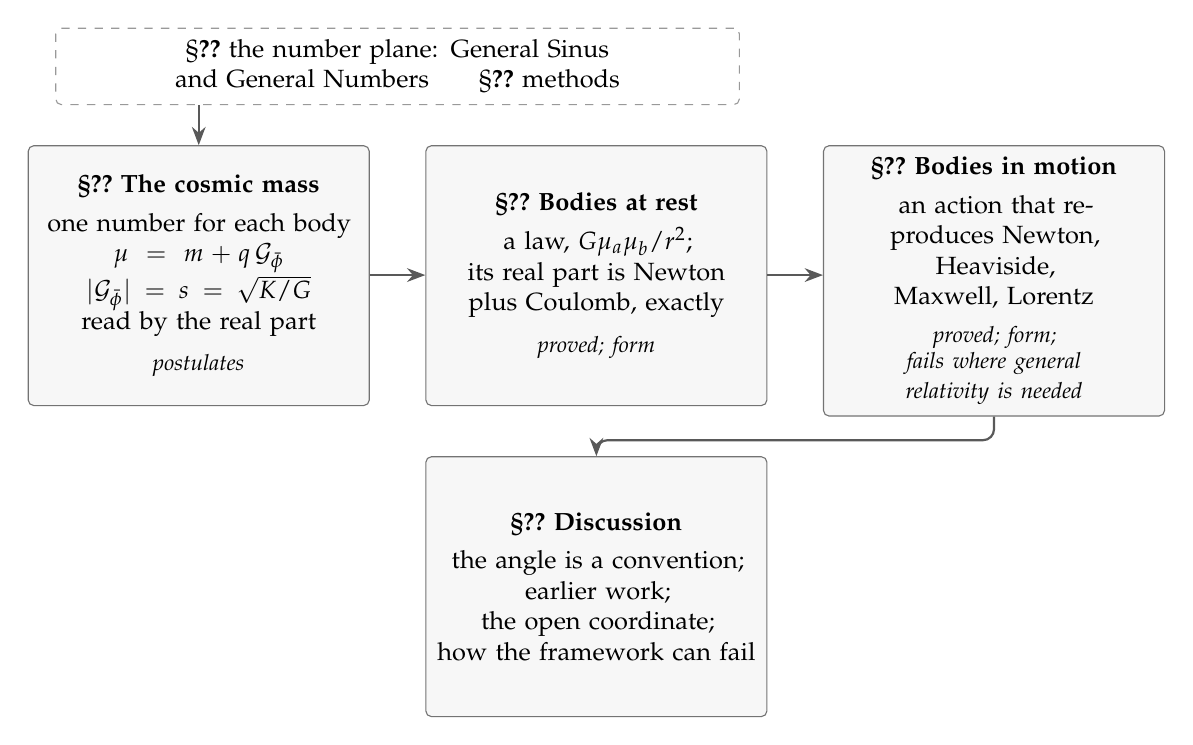
\begin{tikzpicture}[>=Stealth,
  box/.style={draw=black!55, fill=black!3, rounded corners=2pt, text width=4.05cm, align=center, inner sep=4pt, font=\small, minimum height=3.3cm, anchor=north},
  feed/.style={draw=black!40, dashed, rounded corners=2pt, text width=8.4cm, align=center, inner sep=4pt, font=\small},
  flow/.style={->, thick, black!65},
  status/.style={font=\footnotesize\itshape, text=black!60}]
\node[feed] (s23) at (2.525,1.0) {\S\ref{sec:plane} the number plane: General Sinus and General Numbers\qquad \S\ref{sec:methods} methods};
\node[box] (s4) at (0,0) {\textbf{\S\ref{sec:cosmic-mass} The cosmic mass}\\[3pt] one number for each body\\ $\mu = m + q\,\Gp$\\ $|\Gp| = s = \sqrt{K/G}$\\ read by the real part\\[4pt] {\footnotesize\itshape postulates}};
\node[box] (s5) at (5.05,0) {\textbf{\S\ref{sec:rest} Bodies at rest}\\[3pt] a law, $G\mu_a\mu_b/r^2$;\\ its real part is Newton\\ plus Coulomb, exactly\\[4pt] {\footnotesize\itshape proved; form}};
\node[box] (s6) at (10.1,0) {\textbf{\S\ref{sec:motion} Bodies in motion}\\[3pt] an action that\ reproduces Newton,\\ Heaviside, Maxwell, Lorentz\\[4pt] {\footnotesize\itshape proved; form;\\ fails where general\\ relativity is needed}};
\node[box] (s9) at (5.05,-3.95) {\textbf{\S\ref{sec:discussion} Discussion}\\[3pt] the angle is a convention;\\ earlier work;\\ the open coordinate;\\ how the framework can fail};
\draw[flow] (s23.south -| s4.north) -- (s4.north);
\draw[flow] (s4.east |- 0,-1.65) -- (s5.west |- 0,-1.65);
\draw[flow] (s5.east |- 0,-1.65) -- (s6.west |- 0,-1.65);
\draw[flow, rounded corners=4pt] (s6.south) -- ++(0,-0.3) -| (s9.north);
\end{tikzpicture}
\caption{A map of the paper. One number for each body (\cref{sec:cosmic-mass}) is used to write a law for bodies at rest (\cref{sec:rest}) and an action for slow bodies in motion (\cref{sec:motion}); the discussion (\cref{sec:discussion}) shows that the angle of the frame is a convention and states what is left open. The words in italics give the status of each step, as in \cref{tab:glance}.}
\label{fig:map}
\end{figure}

\Cref{sec:plane} recalls the two pieces of mathematics the framework stands on: the General Sinus, a trigonometry of two variables for the oblique triangle~\citep{Derraz2026GSP}, and the General Numbers, whose second axis leans~\citep{DerrazGN2026}. \Cref{sec:methods} gives the constants~\citep{CODATA2022} and the scripts that verify every law and recompute every number printed in the paper. \Cref{sec:cosmic-mass} states the cosmic mass and its reading, and \cref{sec:rest,sec:motion} take the two steps of \cref{fig:map}. \Cref{sec:discussion} separates new content from new form, shows that the angle of the frame is a convention, compares the law with earlier work and with the tests of gravity, and states what is left open and how the framework can fail. \Cref{sec:conclusion} concludes. The electronic supplementary material holds the scripts.

% ======================================================================
\section{The number plane behind the framework}\label{sec:plane}
% ======================================================================

The framework needs two pieces of mathematics, both available as preprints: a trigonometry of two variables for the oblique triangle~\citep{Derraz2026GSP}, and a number plane whose second axis leans~\citep{DerrazGN2026}. This section recalls what the rest of the paper uses, with the number of each statement in those papers.

\subsection{The General Sinus in brief}\label{subsec:gs}

For two angles $\alpha$ and $\phi$ with $\sin(\alpha + \phi) \neq 0$, the general sine, cosine and tangent are~\citep[Definition~3.6 and Theorem~3.7]{Derraz2026GSP}
\begin{equation}\label{eq:gs}
\sin(\alpha, \phi) = \frac{\sin\alpha}{\sin(\alpha + \phi)} , \qquad
\cos(\alpha, \phi) = \frac{\sin\phi}{\sin(\alpha + \phi)} , \qquad
\tan(\alpha, \phi) = \frac{\sin\alpha}{\sin\phi} .
\end{equation}
They return the classical functions when $\alpha + \phi = \pi/2$, and they read coordinates along oblique axes: a unit arrow at the angle $\alpha$ from the first of two axes that meet at the angle $\alpha + \phi$ has the coordinates $\cos(\alpha, \phi)$ and $\sin(\alpha, \phi)$ along them~\citep[Corollary~2.3 and Proposition~2.4]{DerrazGN2026}. They obey the general Pythagoras identity
\begin{equation}\label{eq:gs-pythagoras}
\sin^2(\alpha, \phi) + \cos^2(\alpha, \phi) + 2\sin(\alpha, \phi)\cos(\alpha, \phi)\cos(\alpha + \phi) = 1 ,
\end{equation}
which is the law of cosines of the triangle that the two coordinates make~\citep[Proposition~2.6]{DerrazGN2026}.

\subsection{General Numbers: the relative plane, the Composer Unit and the Axiom}\label{subsec:gn}

A General Number is $w = a + b\,\Gp$, with real numbers $a$ and $b$, where the Composer Unit $\Gp$ is an arrow at the angle $\pb$ to the real axis. One axiom fixes its length by its angle~\citep[Axiom~3.1]{DerrazGN2026}:
\begin{equation}\label{eq:axiom}
\lvert\Gp\rvert = \lvert\cos\pb + \sin\pb\rvert = \sqrt{2}\,\Bigl\lvert\sin\Bigl(\pb + \frac{\pi}{4}\Bigr)\Bigr\rvert .
\end{equation}
For each angle the General Numbers form a relative plane $\GNp$, and the complex plane is the relative plane $\pb = \pi/2$, where $\mathcal{G}_{\pi/2} = i$~\citep[Definition~3.2 and Proposition~3.4]{DerrazGN2026}. Every length $\ell$ with $1 < \ell < \sqrt{2}$ is the length of the Composer Unit at exactly two angles between $0$ and $\pi/2$: the \emph{arcsine root} $\pb_1 = \arcsin(\ell/\sqrt{2}) - \pi/4$ and the \emph{mirror root} $\pb_2 = \pi/2 - \pb_1$~\citep[Theorem~3.6]{DerrazGN2026}. We write $\up = \Gp/\lvert\Gp\rvert$ for the unit arrow along the Composer axis. The \emph{real part} of $w$ is $\Re(w) = a$, its \emph{Composer coordinate} is $b$, and its \emph{Composer part} is $b\,\Gp$~\citep[Definition~3.9]{DerrazGN2026}.

\subsection{The Rule of the Square}\label{subsec:square}

In a relative plane the square of the Composer Unit leans at twice its angle, and its parts are~\citep[Proposition~4.1]{DerrazGN2026}
\begin{equation}\label{eq:square}
\Gp^2 = 2\,\lvert\Gp\rvert\cos\pb\;\Gp - \lvert\Gp\rvert^2 .
\end{equation}
Its real part, $-\lvert\Gp\rvert^2$, is negative at every angle. The product of two General Numbers follows~\citep[Proposition~4.2]{DerrazGN2026}:
\begin{equation}\label{eq:product}
(a + b\,\Gp)(c + d\,\Gp) = \bigl(ac - \lvert\Gp\rvert^2\,bd\bigr) + \bigl(ad + bc + 2\,\lvert\Gp\rvert\cos\pb\;bd\bigr)\Gp .
\end{equation}
Every true relative plane, one with $0 < \pb < \pi$ and $\pb \neq 3\pi/4$~\citep[Definition~3.2]{DerrazGN2026}, is a field, a copy of $\C$ written in an oblique frame~\citep[Proposition~4.3 and Corollary~4.11]{DerrazGN2026}, so every law of complex arithmetic holds in it; what changes is how each law reads in the leaning frame.

\subsection{Two readings of a number: the real part and the shadow}\label{subsec:readings}

Two rules turn a General Number $w = a + b\,\Gp$ into one real number on the real axis~\citep[Definitions~3.9 and~3.10]{DerrazGN2026}. The \emph{real part} $\Re(w) = a$ walks back to the real axis along the Composer axis, the way the number was built. The \emph{shadow} drops the tip straight down,
\begin{equation}\label{eq:shadow}
\Sh(w) = a + b\,\lvert\Gp\rvert\cos\pb , \qquad \Ht(w) = b\,\lvert\Gp\rvert\sin\pb ,
\end{equation}
where $\Ht(w)$ is the height above the real axis. The two readings agree on real numbers and differ as soon as $b \neq 0$.

% ======================================================================
\section{Methods}\label{sec:methods}
% ======================================================================

\subsection{Constants and units}\label{subsec:constants}

All constants are the CODATA 2022 recommended values~\citep{CODATA2022}, in SI units: $G = 6.67430(15) \times 10^{-11}$~m$^3$\,kg$^{-1}$\,s$^{-2}$, $K = 1/(4\pi\varepsilon_0)$ with $\varepsilon_0 = 8.8541878188(14) \times 10^{-12}$~F\,m$^{-1}$, the exact $c$ and $e$, the masses of the electron, the proton and the neutron, the fine-structure constant, the Bohr radius and the Rydberg energy. The size of the Composer Unit, $s = \lvert\Gp\rvert = \sqrt{K/G} \approx 1.16043 \times 10^{10}$~kg\,C$^{-1}$, is known to about one part in $10^5$, half the relative uncertainty of $G$. No measured quantity of this paper depends on the angle of the Composer axis (\cref{subsec:angle-units}). Where a figure or a number of the frame needs an angle, we read $s$ in units of $10^{10}$~kg\,C$^{-1}$ (\cref{subsec:our-plane}), which gives the mirror root $79.8605^\circ$ of the Axiom; one standard error of $G$ moves it by $0.0009^\circ$. We hold the angle at $\pb = 79.86^\circ$, as in the worked examples of~\citep{DerrazGN2026}.

\subsection{Verification and scripts}\label{subsec:scripts}

A Python script, given in the electronic supplementary material, checks the paper. \texttt{verify\_cmt.py} checks every numbered statement, symbolically with SymPy~\citep{Meurer2017} where it is algebra or calculus and numerically otherwise, recomputes every computed number printed in the paper, and ends with a coverage check that every numbered statement of the paper has at least one check. Values taken from the literature are checked only as printed. On the text submitted here, \texttt{verify\_cmt.py} passes all 106 of its checks: 41 symbolic, 9 numerical and 55 printed values, and the coverage check of the 34 numbered statements and labelled equations.

% ======================================================================
\section{The cosmic mass}\label{sec:cosmic-mass}
% ======================================================================

\emph{What number can carry a mass and a charge at once?} This section proposes one number for each body, fixes the size of its second unit from two measured constants, says which angle the frame is drawn at and why that choice is free, and says how the number is read. The statements that the paper assumes are labelled postulates: the two of this section, and the two laws of \cref{sec:rest,sec:motion}.

\subsection{One number for mass and charge}\label{subsec:cm-def}

\begin{postulate}[Cosmic mass]\label{def:cosmic-mass}
The \emph{cosmic mass} of a body of mass $m$ and electric charge $q$ is the General Number
\[
\mu = m + q\,\Gp ,
\]
in kilograms. Its real part is the mass $m$, its Composer coordinate is the charge $q$, and its Composer part $q\,\Gp$, the \emph{charge part}, is in kilograms, so that the Composer Unit $\Gp$ carries the unit kg\,C$^{-1}$.
\end{postulate}

\begin{figure}[t]
\centering
% The cosmic mass as a General Number (Postulate 4.1). Drawn at 55 degrees, not 79.86, so that the lean is visible.
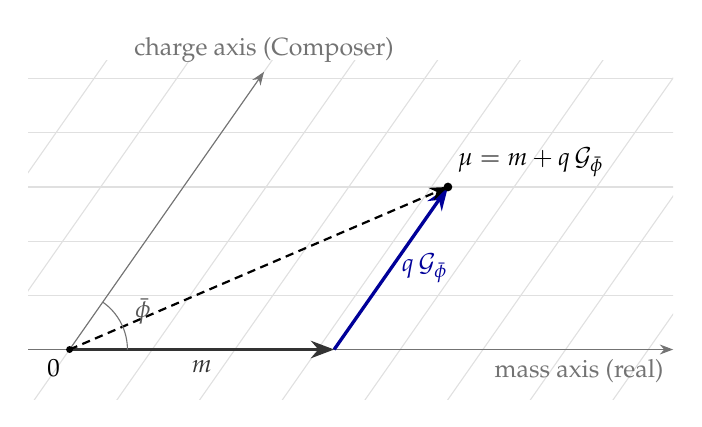
\begin{tikzpicture}[>=Stealth, scale=1.05, every node/.style={font=\small}]
  \def\ang{55}
  \begin{scope}
    \clip (-0.5,-0.6) rectangle (7.3,3.5);
    \foreach \a in {-3,...,7} \draw[black!12] ($(\a,0)+(\ang:-2)$) -- ($(\a,0)+(\ang:6)$);
    \foreach \b in {-1,...,5} \draw[black!12] ($(-3,0)+(\ang:{\b*0.8})$) -- ($(9,0)+(\ang:{\b*0.8})$);
  \end{scope}
  \draw[->, black!55] (-0.5,0) -- (7.3,0) node[below left] {mass axis (real)};
  \draw[->, black!55] (0,0) -- (\ang:4.1) node[above] {charge axis (Composer)};
  \draw[->, very thick, black!80] (0,0) -- (3.2,0) node[midway, below] {$m$};
  \draw[->, very thick, blue!60!black] (3.2,0) -- ($(3.2,0)+(\ang:2.4)$) node[midway, right] {$q\,\Gp$};
  \draw[->, thick, densely dashed] (0,0) -- ($(3.2,0)+(\ang:2.4)$);
  \fill ($(3.2,0)+(\ang:2.4)$) circle (1.5pt) node[above right] {$\mu = m + q\,\Gp$};
  \draw[black!55] (0.7,0) arc (0:\ang:0.7);
  \node[black!65] at ({\ang/2}:1.0) {$\pb$};
  \fill (0,0) circle (1.2pt) node[below left] {$0$};
\end{tikzpicture}

\caption{The cosmic mass of a body as a General Number (\cref{def:cosmic-mass}): $m$ steps along the mass axis and $q$ steps of the Composer Unit along the charge axis. The charge axis is drawn at $55^\circ$ and the two parts with comparable lengths, so that the construction can be seen; the paper's frame is drawn at $79.86^\circ$, and for a charged particle the charge part is about $10^{18}$ to $10^{21}$ times longer than the mass.}
\label{fig:cosmic-mass}
\end{figure}

\Cref{fig:cosmic-mass} draws the construction. A neutral body is a real cosmic mass. The free neutron, for example, is the real number $\mu_n = m_n$. A body with charge has a second part, and for the elementary particles that part dominates. With the size of the Composer Unit found below, the charge part of the electron, $e\,\lvert\Gp\rvert \approx 1.85921 \times 10^{-9}$~kg, is about $2.04 \times 10^{21}$ times its mass, and that of the proton about $1.11 \times 10^{18}$ times its mass.

\subsection{The size and the angle of the Composer Unit}\label{subsec:our-plane}

The Composer Unit has a size and an angle. The size is a physical quantity; the angle, as we shall see, belongs to the frame in which the plane is drawn. The size is fixed by asking that the term of two charges in the product of two cosmic masses (\cref{sec:rest}) have the strength of Coulomb's law:
\begin{equation}\label{eq:cu-size}
G\,s^2 = K , \qquad s = \lvert\Gp\rvert = \sqrt{\frac{K}{G}} = c\,\sqrt{\frac{\mu_0}{4\pi G}} \approx 1.16043 \times 10^{10}\ \mathrm{kg\,C^{-1}} ,
\end{equation}
where the second form uses $K = \mu_0 c^2/(4\pi)$, with $\mu_0$ the magnetic constant. This is Stoney's ratio of mass to charge~\citep{Stoney1881}. With the CODATA 2022 values~\citep{CODATA2022} it is known to about one part in $10^5$, half the relative uncertainty of $G$. The constant $K$ therefore enters the framework as an input; the Coulomb term has Coulomb's strength because $s$ was chosen to give it.

The Axiom~\cref{eq:axiom} compares the length of the Composer Unit with the pure number $\lvert\cos\pb + \sin\pb\rvert$, while $s$ carries the unit kg\,C$^{-1}$. To give it an angle, a scale unit $u$ must first be chosen, and the Axiom is read for the pure number $A = s/u$. With $u = 10^{10}$~kg\,C$^{-1}$, $A = 1.16043$ and
\begin{equation}\label{eq:our-angle}
\lvert\cos\pb + \sin\pb\rvert = A = 1.16043 .
\end{equation}
We keep the two symbols apart: $s$ is the physical size, fixed by the measured constants $G$ and $K$, and $A$ is the drawing length, fixed by the choice of $u$.
By \citep[Theorem~3.6]{DerrazGN2026}, two angles between $0$ and $\pi/2$ satisfy~\cref{eq:our-angle}:
\[
\pb_1 = \arcsin\Bigl(\frac{1.16043}{\sqrt{2}}\Bigr) - \frac{\pi}{4} \approx 10.14^\circ , \qquad \pb_2 = \frac{\pi}{2} - \pb_1 \approx 79.86^\circ .
\]
We draw the frame at the mirror root, $\pb = 79.8605^\circ$, held at $79.86^\circ$ as in the worked examples of~\citep{DerrazGN2026}, for which $\sin\pb \approx 0.98438$ and $\cos\pb \approx 0.17605$; \cref{subsec:why-sign} says why this root is the natural one to draw. Both the scale unit and the root are conventions. In units of $10^{9}$~kg\,C$^{-1}$ the drawing length would be $11.6$, and the Axiom would have no root; in Planck or Stoney units it is $1$, and the Axiom returns the right angle of the complex plane. \Cref{subsec:angle-units} shows that no measured quantity depends on the choice.

\subsection{The real reading}\label{subsec:real-reading}

A product of two cosmic masses is a General Number, while an instrument returns one real number. We fix the rule once.

\begin{postulate}[The real reading]\label{def:real-reading}
Every measured force, energy and momentum is the real part of a General Number. The Composer coordinate of a force, an energy or a momentum is not read as a measured quantity.
\end{postulate}

The shadow~\cref{eq:shadow} is the other natural rule. For a neutral body the two agree; \cref{subsec:why-sign} shows where they part and why the framework reads by the real part. \Cref{tab:dictionary} sets the words of the General Numbers beside the names they take for the cosmic mass.

\begin{table}[t]
\caption{One object, two vocabularies. On the left, the words of the General Numbers, with the statement of~\citep{DerrazGN2026} that defines each one; on the right, their names for the cosmic mass in this paper.}
\label{tab:dictionary}
\small
\begin{tabularx}{\textwidth}{@{}>{\raggedright\arraybackslash}p{0.44\textwidth}c>{\raggedright\arraybackslash}X@{}}
\toprule
General Numbers & \citep{DerrazGN2026} & cosmic mass \\
\midrule
General Number $w = a + b\,\Gp$ & Ax.~3.1 & cosmic mass $\mu = m + q\,\Gp$ \\
real axis; Composer axis & Ax.~3.1 & mass axis; charge axis \\
real part $\Re(w) = a$ & Def.~3.9 & mass $m$ \\
Composer coordinate $b$ & Def.~3.9 & charge $q$ \\
Composer part $b\,\Gp$ & Def.~3.9 & charge part $q\,\Gp$, in kilograms \\
length of the Composer Unit & Ax.~3.1 & size $s = \sqrt{K/G}$; drawing length $A = s/u$ in a chosen unit $u$ \\
real number; pure Composer number & Def.~3.9 & neutral body; a charge without mass \\
real part of a product & Prop.~4.2 & every measured force, energy and momentum \\
Rule of the Square, $\Re(\Gp^2) = -\lvert\Gp\rvert^2$ & Prop.~4.1 & the minus sign between gravity and Coulomb's force, at every angle \\
mirror root & Thm~3.6 & the angle $79.86^\circ$ at which the frame is drawn, for $u = 10^{10}$~kg\,C$^{-1}$ \\
\bottomrule
\end{tabularx}
\end{table}

% ======================================================================
\section{Bodies at rest: the Cosmic Interaction Law}\label{sec:rest}
% ======================================================================

\emph{What happens when two cosmic masses meet?} This section proposes a law for a pair of bodies at rest, reads it in its own plane, and recovers Newton's and Coulomb's laws, with the sign that makes like charges push apart.

\subsection{Two numbers, two laws}\label{subsec:two-numbers}

Classical physics describes two bodies $a$ and $b$, at the distance $r$, by two numbers each: the masses $m_a$, $m_b$ in kilograms and the charges $q_a$, $q_b$ in coulombs. Along the unit arrow $\er$ from $a$ to $b$ it writes two laws of one shape, Newton's with the constant $G$ and Coulomb's with the constant $K$~\cref{eq:two-laws}. We write each force along the line as a signed number: a positive value is a pull, a negative value a push. Gravity is then $+G\,m_a m_b/r^2$, and electricity is $-K\,q_a q_b/r^2$, a push for like charges.

\subsection{The interaction law}\label{subsec:one-law}

\begin{postulate}[The Cosmic Interaction Law]\label{law:interaction}
Two bodies with the cosmic masses $\mu_a = m_a + q_a\Gp$ and $\mu_b = m_b + q_b\Gp$, at the distance $r$, interact by
\[
\vec{F}_G = G\cdot\frac{\mu_a\mu_b}{r^2}\cdot\er .
\]
Expanded, the law has three terms:
\begin{align*}
\vec{F}_G &= G\cdot\frac{m_a m_b}{r^2}\cdot\er
 + \Gp^2\cdot G\cdot\frac{q_a q_b}{r^2}\cdot\er
 + \Gp\cdot G\cdot\frac{m_a q_b + q_a m_b}{r^2}\cdot\er .
\end{align*}
\end{postulate}

Like the two postulates of \cref{sec:cosmic-mass}, the law is assumed. The rest of this section works out how it reads. We keep the name Cosmic Interaction Law for it. The first term is Newton's law. The second has the shape of Coulomb's law, scaled by $\Gp^2$. The third mixes the mass of each body with the charge of the other; we call it the \emph{Coupling term}. For two protons one metre apart, the three terms have the sizes $1.87 \times 10^{-64}$~N, $2.31 \times 10^{-28}$~N and $4.15 \times 10^{-46}$~N, the last read as the length of its Composer part.

\subsection{Reading the law by its real part}\label{subsec:reading-law}

\begin{proposition}[The real part of the interaction law]\label{prop:law-real}
In the relative plane of the Composer Unit, the product of two cosmic masses is
\[
\mu_a\mu_b = \bigl(m_a m_b - \lvert\Gp\rvert^2\,q_a q_b\bigr) + \bigl(m_a q_b + q_a m_b + 2\,\lvert\Gp\rvert\cos\pb\;q_a q_b\bigr)\Gp ,
\]
and its real part, multiplied by $G$, is
\[
G\,\Re(\mu_a\mu_b) = G\,m_a m_b - K\,q_a q_b .
\]
The Coupling term has no real part, and the angle $\pb$ appears only in the Composer coordinate.
\end{proposition}

\begin{proof}
Multiply out, $\mu_a\mu_b = m_a m_b + (m_a q_b + q_a m_b)\,\Gp + q_a q_b\,\Gp^2$, and replace $\Gp^2$ by the Rule of the Square~\cref{eq:square}; this is the product~\cref{eq:product} with $a, b, c, d = m_a, q_a, m_b, q_b$. The real part is the first bracket, and $G\,\lvert\Gp\rvert^2 = K$ by~\cref{eq:cu-size}.
\end{proof}

\begin{definition}[Reading the law]\label{def:reading}
The force that the Cosmic Interaction Law exerts along $\er$ is the real part of the law,
\[
F = G\cdot\frac{\Re(\mu_a\mu_b)}{r^2} = G\cdot\frac{m_a m_b}{r^2} - K\cdot\frac{q_a q_b}{r^2} ,
\]
a pull when it is positive and a push when it is negative. The Composer coordinate of $\mu_a\mu_b$ is not read as a force.
\end{definition}

\begin{figure}[t]
\centering
% The product of two cosmic masses as four rectangles (Law 5.1 and Proposition 5.2). Not to scale.
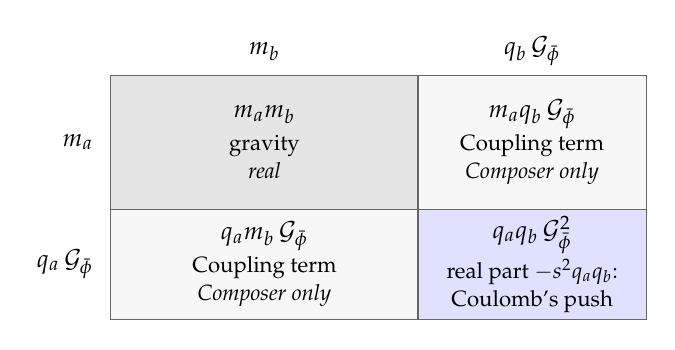
\begin{tikzpicture}[every node/.style={font=\small}]
  \def\wa{3.9}\def\wb{2.9}\def\ha{1.7}\def\hb{1.4}
  \fill[black!10] (0,0) rectangle (\wa,\ha);
  \fill[black!3] (\wa,0) rectangle ({\wa+\wb},\ha);
  \fill[black!3] (0,-\hb) rectangle (\wa,0);
  \fill[blue!12] (\wa,-\hb) rectangle ({\wa+\wb},0);
  \draw[black!60] (0,-\hb) rectangle ({\wa+\wb},\ha);
  \draw[black!60] (\wa,-\hb) -- (\wa,\ha);
  \draw[black!60] (0,0) -- ({\wa+\wb},0);
  \node at ({\wa/2},{\ha+0.3}) {$m_b$};
  \node at ({\wa+\wb/2},{\ha+0.3}) {$q_b\,\Gp$};
  \node[anchor=east] at (-0.1,{\ha/2}) {$m_a$};
  \node[anchor=east] at (-0.1,{-\hb/2}) {$q_a\,\Gp$};
  \node[align=center] at ({\wa/2},{\ha/2}) {$m_a m_b$\\[1pt] {\footnotesize gravity}\\[-1pt] {\footnotesize\itshape real}};
  \node[align=center] at ({\wa+\wb/2},{\ha/2}) {$m_a q_b\,\Gp$\\[1pt] {\footnotesize Coupling term}\\[-1pt] {\footnotesize\itshape Composer only}};
  \node[align=center] at ({\wa/2},{-\hb/2}) {$q_a m_b\,\Gp$\\[1pt] {\footnotesize Coupling term}\\[-1pt] {\footnotesize\itshape Composer only}};
  \node[align=center] at ({\wa+\wb/2},{-\hb/2}) {$q_a q_b\,\Gp^2$\\[1pt] {\footnotesize real part $-s^2 q_a q_b$:}\\[-1pt] {\footnotesize Coulomb's push}};
\end{tikzpicture}

\caption{The product of two cosmic masses, multiplied out as four rectangles (\cref{law:interaction,prop:law-real}). Mass times mass gives gravity. Each mass times the other body's charge gives the Coupling term, which lies along the Composer axis and has no real part. Charge times charge gives $q_a q_b\,\Gp^2$, whose real part is $-s^2 q_a q_b$ by the Rule of the Square: Coulomb's push, at every angle. The pieces are not drawn to scale.}
\label{fig:product}
\end{figure}

This is the real reading of \cref{def:real-reading} applied to one law (\cref{fig:product}). It reproduces Newton's and Coulomb's laws together, each with its own constant and its own sign, and adds nothing to them: a body at rest feels no new force.

\subsection{Why like charges push apart, at every angle}\label{subsec:why-sign}

In this framework the sign in \cref{def:reading} comes from the algebra of the plane. Had mass and charge been put into one real number, $\mu = m + \lambda q$ with a real $\lambda$ in kg\,C$^{-1}$, the product would be $\mu_a\mu_b = m_a m_b + \lambda(m_a q_b + q_a m_b) + \lambda^2 q_a q_b$. Since $\lambda^2 > 0$ for every $\lambda$, a law built on that product would pull two like charges together exactly as it pulls two masses. The choice $\lambda^2 = K/G$ gives the electric term Coulomb's strength, but no choice of $\lambda$ gives it Coulomb's sign. To carry both signs, the law needs a unit whose square points back along the mass axis.

\begin{proposition}[The sign of the interaction]\label{prop:sign}
In every true relative plane, whatever the angle $\pb$, the real part of the Cosmic Interaction Law is
\[
F = \frac{G\,m_a m_b - K\,q_a q_b}{r^2} .
\]
Two masses pull, two like charges push, and two unlike charges pull, each with the full strength of Newton's or Coulomb's law.
\end{proposition}

\begin{proof}
By the Rule of the Square~\cref{eq:square}, $\Re(\Gp^2) = -s^2$ for every $\pb$, so \cref{prop:law-real} holds with no condition on the angle; the signs follow from those of $m_a m_b \ge 0$ and of $q_a q_b$.
\end{proof}

The sign rests on one choice, the real reading (\cref{def:real-reading}); read by the shadow instead, it would depend on the angle (below).
 Given that reading, the minus sign is not put in by hand: it is the real coordinate of the square of the second unit, $-s^2$, which the Rule of the Square gives for every angle and every length~\citep[Proposition~4.1]{DerrazGN2026}. A reader may still say that writing a pair $(m, q)$ with the quadratic form $m_a m_b - s^2 q_a q_b$ builds the sign in, as a metric with one plus and one minus would. Our only reply is that here the form is the multiplication of a number system, a field, so that every rule of complex arithmetic applies to it (\cref{subsec:square,subsec:why-lean}); whether this is more than a choice of notation, the reader may judge.

\paragraph{Which root to draw.} The angle enters only through the other reading. By~\cref{eq:shadow}, the shadow of $\Gp$ is $\lvert\Gp\rvert\cos\pb$ and the shadow of $\Gp^2$ is $\lvert\Gp\rvert^2\cos 2\pb$, so that
\begin{equation}\label{eq:shadow-law}
G\,\Sh(\mu_a\mu_b) = G\,m_a m_b + \sqrt{KG}\,\cos\pb\,(m_a q_b + q_a m_b) + K\cos 2\pb\;q_a q_b .
\end{equation}
Read by its shadow, the electric term keeps only the share $\cos 2\pb$ of Coulomb's strength, and for like charges it has the sign of $\cos 2\pb$. At the arcsine root, $\cos 2\pb_1 \approx 0.93801$, and two like charges would pull. At the mirror root, $\cos 2\pb_2 \approx -0.93801$, the square of the Composer Unit leans at $159.72^\circ$ and points back along the mass axis, as it does for every angle between $\pi/4$ and $3\pi/4$~\citep[Theorem~3.7]{DerrazGN2026}, and like charges push in both readings. We therefore draw the frame at the mirror root, $\pb = 79.86^\circ$. The choice is a convention. The real reading, which is the one this paper uses (\cref{def:real-reading}), gives Coulomb's full strength and sign at every angle (\cref{prop:sign}), and at the drawn angle the shadow reading is excluded by experiment (\cref{subsec:coupling}). As far as this paper goes, the angle fixes only the Composer coordinate and the drawing of the frame.



% ======================================================================
\section{Bodies in motion: the Cosmic Field Law}\label{sec:motion}
% ======================================================================

\emph{What does the law become when the bodies move?} Maxwell joined electricity and magnetism in one field~\citep{Maxwell1865}, and Heaviside wrote gravity in Maxwell's form~\citep{Heaviside1893}. This section asks whether the same road can be walked from the other end: from one number for each body to a field, and to an action.

\subsection{The cosmic mass in motion}\label{subsec:un-reading}

In this framework every body carries its cosmic mass $\mu = m + q\,\Gp$, and every measurement is read by the real part (\cref{def:real-reading}). The products that matter are of one kind: by~\cref{eq:product}, for real coefficients,
\begin{equation}\label{eq:real-product}
\Re\bigl[(a + b\,\Gp)(c + d\,\Gp)\bigr] = ac - \lvert\Gp\rvert^2\,bd ,
\end{equation}
which does not depend on the angle. Matter in motion is described by the density and the current of cosmic mass, $\rho_\mu = \rho_m + \rho_q\,\Gp$ and $\vJ_\mu = \vJ_m + \vJ_q\,\Gp$, built from the densities and currents of mass and charge.

\subsection{From forces to fields}\label{subsec:un-fields}

\begin{definition}[The cosmic field of a body at rest]\label{def:un-field}
A body of cosmic mass $\mu_s$ at rest at the origin makes, at the distance $r$ in the outward direction $\rhat$, the \emph{cosmic field}
\[
\uE = -\frac{G\mu_s}{r^2}\,\rhat .
\]
Its value at each point is a vector with General Number components, $\uE = \vg + \ve\,\Gp$.
\end{definition}

A second body of cosmic mass $\mu$ at that point feels $\Re(\mu\,\uE) = -G\,\Re(\mu\,\mu_s)\,\rhat/r^2$, the Cosmic Interaction Law read by its real part (\cref{def:reading}): a pull towards the source when $G\,\Re(\mu\mu_s) > 0$. Fields that change in time need a second field, as in Maxwell's theory.

\subsection{The Cosmic Field Law}\label{subsec:un-law}

\begin{postulate}[The Cosmic Field Law]\label{law:unified}
Two fields with General Number values, the cosmic field $\uE$ and the second field $\uB$, obey
\begin{align*}
\text{(F1)}\quad \nabla\cdot\uE &= -4\pi G\,\rho_\mu , & \text{(F2)}\quad \nabla\cdot\uB &= 0 ,\\
\text{(F3)}\quad \nabla\times\uE &= -\partial_t\uB , & \text{(F4)}\quad \nabla\times\uB &= -\frac{4\pi G}{c^2}\vJ_\mu + \frac{1}{c^2}\partial_t\uE ,
\end{align*}
and a body of cosmic mass $\mu$ and velocity $\vv$ moves by
\[
\text{(M)}\qquad \Re(\mu)\,\frac{d\vv}{dt} = \Re\bigl[\mu\,(\uE + \vv\times\uB)\bigr] .
\]
\end{postulate}

Like \cref{law:interaction}, \cref{law:unified} is assumed. It is Maxwell's set of equations written for fields with General Number values, with the constant $4\pi G$ fixed by the field of a body at rest. The statements below are derived from it.

\subsection{The split: gravity with a small magnetic part, Maxwell's equations, and waves at \texorpdfstring{$c$}{c}}\label{subsec:un-split}

Write $\uB = \vB_g + \vb\,\Gp$, as $\uE = \vg + \ve\,\Gp$.

\begin{proposition}[The split]\label{prop:un-split}
Each of the field equations (F1) to (F4) holds separately for the real coordinate and for the Composer coordinate, as in \cref{tab:un-split}.
\end{proposition}

\begin{proof}
Every operation in (F1) to (F4) is a sum, a product by a real number, or a derivative in space or time; no field multiplies a field, and no field is multiplied by $\Gp$. Each such operation acts on the two coordinates one at a time, and two General Numbers are equal exactly when both coordinates are equal~\citep[Remark~3.3]{DerrazGN2026}. So each equation is two equations.
\end{proof}

\begin{table}[t]
\caption{The four field equations of \cref{law:unified}, split into their two coordinates (\cref{prop:un-split}). The angle $\pb$ appears in neither set.}
\label{tab:un-split}
\small\centering
\begin{tabular}{@{}ll@{}}
\toprule
real coordinate & Composer coordinate \\
\midrule
$\nabla\cdot\vg = -4\pi G\rho_m$ & $\nabla\cdot\ve = -4\pi G\rho_q$ \\[2pt]
$\nabla\cdot\vB_g = 0$ & $\nabla\cdot\vb = 0$ \\[2pt]
$\nabla\times\vg = -\partial_t\vB_g$ & $\nabla\times\ve = -\partial_t\vb$ \\[2pt]
$\nabla\times\vB_g = -\frac{4\pi G}{c^2}\vJ_m + \frac{1}{c^2}\partial_t\vg$ & $\nabla\times\vb = -\frac{4\pi G}{c^2}\vJ_q + \frac{1}{c^2}\partial_t\ve$ \\
\bottomrule
\end{tabular}
\end{table}

The real set is Newton's gravity with a second field. For bodies at rest, (F3) gives $\vg$ no curl and (F1) gives the field of a mass $M$, $\vg = -GM\rhat/r^2$. The field $\vB_g$, made by moving masses and felt by moving masses, is the magnetic part of gravity that Heaviside wrote in 1893~\citep{Heaviside1893}.

\begin{theorem}[Maxwell's equations]\label{thm:un-maxwell}
Define the electric and magnetic fields by
\[
\vE = -\lvert\Gp\rvert^2\,\ve , \qquad \vB = -\lvert\Gp\rvert^2\,\vb .
\]
Then the Composer set of \cref{tab:un-split} is Maxwell's set,
\begin{align*}
\nabla\cdot\vE &= 4\pi K\rho_q , & \nabla\cdot\vB &= 0 ,\\
\nabla\times\vE &= -\partial_t\vB , & \nabla\times\vB &= \frac{4\pi K}{c^2}\vJ_q + \frac{1}{c^2}\partial_t\vE ,
\end{align*}
with the magnetic constant $\mu_0 = 4\pi K/c^2$.
\end{theorem}

\begin{proof}
Multiply each Composer equation by $-\lvert\Gp\rvert^2$ and use $G\,\lvert\Gp\rvert^2 = K$~\cref{eq:cu-size}. With $K = 1/(4\pi\varepsilon_0)$ and $\mu_0 = 4\pi K/c^2$ these are Maxwell's equations in SI form.
\end{proof}

The minus sign in the definition of $\vE$ turns the arrows round, so that the field of a mass points in while Maxwell's field of a positive charge points out (\cref{fig:fields}).

\begin{figure}[t]
\centering
% The cosmic field of one source at rest in its two coordinates (Definition 6.1 and Theorem 6.4).
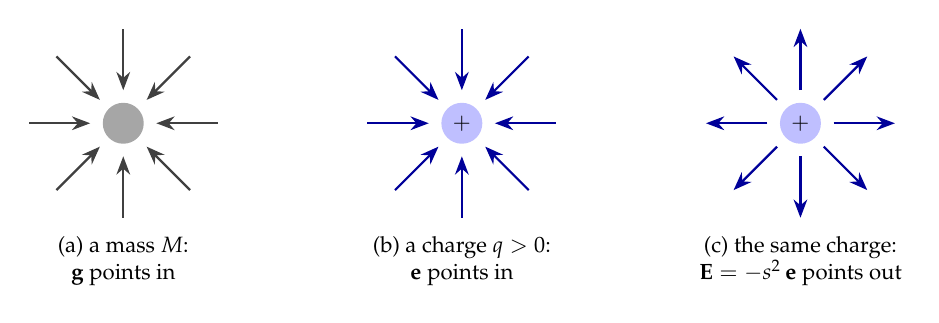
\begin{tikzpicture}[>=Stealth, font=\footnotesize]
  \begin{scope}
    \foreach \a in {0,45,...,315} \draw[<-, thick, black!75] (\a:0.42) -- (\a:1.2);
    \fill[black!35] (0,0) circle (0.26);
    \node[align=center] at (0,-1.75) {(a) a mass $M$:\\ $\vg$ points in};
  \end{scope}
  \begin{scope}[xshift=4.3cm]
    \foreach \a in {0,45,...,315} \draw[<-, thick, blue!60!black] (\a:0.42) -- (\a:1.2);
    \fill[blue!25] (0,0) circle (0.26); \node at (0,0) {$+$};
    \node[align=center] at (0,-1.75) {(b) a charge $q > 0$:\\ $\ve$ points in};
  \end{scope}
  \begin{scope}[xshift=8.6cm]
    \foreach \a in {0,45,...,315} \draw[->, thick, blue!60!black] (\a:0.42) -- (\a:1.2);
    \fill[blue!25] (0,0) circle (0.26); \node at (0,0) {$+$};
    \node[align=center] at (0,-1.75) {(c) the same charge:\\ $\vE = -s^2\,\ve$ points out};
  \end{scope}
\end{tikzpicture}

\caption{The cosmic field $\uE = -G\mu_s\rhat/r^2$ of one source at rest, in its two coordinates (\cref{def:un-field,thm:un-maxwell}). (a) The real coordinate $\vg$ of a mass points inward: Newton's pull. (b) The Composer coordinate $\ve$ of a positive charge points inward too, by the same formula. (c) Maxwell's field of that charge, $\vE = -s^2\,\ve$, points outward. The minus sign of the Rule of the Square turns the arrows round: masses pull, and like charges push.}
\label{fig:fields}
\end{figure}

\begin{theorem}[Waves at the speed $c$]\label{thm:un-waves}
In empty space both fields obey the wave equation with the speed $c$,
\[
\nabla^2\uE = \frac{1}{c^2}\,\partial_t^2\uE , \qquad \nabla^2\uB = \frac{1}{c^2}\,\partial_t^2\uB ,
\]
in both coordinates: the waves of the gravity part travel at the speed of light.
\end{theorem}

\begin{proof}
With no sources, take the curl of (F3) and use $\nabla\times(\nabla\times\vF) = \nabla(\nabla\cdot\vF) - \nabla^2\vF$, then (F4) and (F1): $\nabla(\nabla\cdot\uE) - \nabla^2\uE = -c^{-2}\partial_t^2\uE$ with $\nabla\cdot\uE = 0$. The curl of (F4), with (F3) and (F2), gives the equation for $\uB$. By \cref{prop:un-split} each equation holds for both coordinates.
\end{proof}

The gravitational waves of the neutron-star merger GW170817 arrived within two seconds of its gamma rays after about 130 million years, which ties the speed of gravity to the speed of light within a few parts in $10^{15}$~\citep{Abbott2017GRB}. This agrees with \cref{thm:un-waves}, though only as a check of consistency, since the speed $c$ was put into (F4) for both coordinates. The inspiral that sent those waves contradicts the sign of their energy (\cref{subsec:un-limits}).

\subsection{Motion: the two coordinates of the law of motion}\label{subsec:un-motion}

\begin{proposition}[The law of motion in its two coordinates]\label{prop:un-lorentz}
Opened into its coordinates, the law of motion (M) reads
\[
m\,\frac{d\vv}{dt} = m\,(\vg + \vv\times\vB_g) + q\,(\vE + \vv\times\vB) .
\]
\end{proposition}

\begin{proof}
By~\cref{eq:real-product}, applied to each component, with $\mu = m + q\,\Gp$ and $\uE = \vg + \ve\,\Gp$, $\Re(\mu\,\uE) = m\,\vg - \lvert\Gp\rvert^2 q\,\ve = m\,\vg + q\,\vE$. In the same way, with $\vv$ real, $\Re(\mu\,\vv\times\uB) = m\,\vv\times\vB_g + q\,\vv\times\vB$. The left side of (M) is $\Re(\mu)\,d\vv/dt = m\,d\vv/dt$.
\end{proof}

The first bracket is Newton's gravity with Heaviside's magnetic part; the second is the force of Lorentz~\citep{Lorentz1895}. The mass that resists acceleration is the real part of the cosmic mass, and the Coupling term of \cref{law:interaction} exerts no force.

\paragraph{Free fall.} The law of motion keeps the equivalence of the mass that falls and the mass that resists. In the field $\vg$ of a neutral source, a body of cosmic mass $m + q\,\Gp$ at rest feels $\Re(\mu\,\uE) = m\,\vg$, since the field has no Composer coordinate, and its inertia is $m$; so $d\vv/dt = \vg$ for every body, whatever its mass, its charge or its make-up. The charge of a body enters only through the Composer coordinate of the field, which a neutral source does not make. This agrees with the equality of free fall measured to about one part in $10^{15}$ by MICROSCOPE~\citep{Touboul2022}, and it is the same statement as in Newton's mechanics: the law adds nothing to it.

\subsection{What is kept: the source, the energy and the momentum}\label{subsec:un-kept}

\begin{theorem}[Conservation of the source]\label{thm:un-source}
The density and the current of cosmic mass obey $\partial_t\rho_\mu + \nabla\cdot\vJ_\mu = 0$.
\end{theorem}

\begin{proof}
Take the divergence of (F4). The left side is zero, since $\nabla\cdot(\nabla\times\vF) = 0$; replace $\nabla\cdot\uE$ by (F1) and divide by $-4\pi G/c^2$.
\end{proof}

The Composer coordinate of \cref{thm:un-source} is the conservation of charge, which holds exactly. The real coordinate says that rest mass is conserved. The law therefore cannot describe a process that turns rest mass into energy, such as a nuclear fusion, whose energy comes from special relativity.

\begin{theorem}[The balance of energy]\label{thm:un-energy}
Let
\[
u = -\frac{1}{8\pi G}\,\Re\bigl[\uE\cdot\uE + c^2\,\uB\cdot\uB\bigr], \qquad \vS = -\frac{c^2}{4\pi G}\,\Re\bigl[\uE\times\uB\bigr].
\]
Then $\partial_t u + \nabla\cdot\vS = -\Re\bigl[\uE\cdot\vJ_\mu\bigr]$.
\end{theorem}

\begin{proof}
By $\nabla\cdot(\vF\times\vH) = \vH\cdot(\nabla\times\vF) - \vF\cdot(\nabla\times\vH)$ with (F3) and (F4),
$\nabla\cdot(\uE\times\uB) = -\tfrac12\partial_t(\uB\cdot\uB) - \tfrac{1}{2c^2}\partial_t(\uE\cdot\uE) + \tfrac{4\pi G}{c^2}\,\uE\cdot\vJ_\mu$. Take the real part and multiply by $-c^2/(4\pi G)$.
\end{proof}

\begin{proposition}[The energy in its two coordinates]\label{prop:un-two-faces}
Opened into its coordinates, the energy density of \cref{thm:un-energy} is
\[
u = -\frac{g^2 + c^2 B_g^2}{8\pi G} + \frac{E^2 + c^2 B^2}{8\pi K} :
\]
negative for the gravity part and positive for the Maxwell part.
\end{proposition}

\begin{proof}
By~\cref{eq:real-product}, with $\ve = -\vE/\lvert\Gp\rvert^2$, $\Re[\uE\cdot\uE] = g^2 - \lvert\Gp\rvert^2 e^2 = g^2 - E^2/\lvert\Gp\rvert^2$. Multiply by $-1/(8\pi G)$, use $G\,\lvert\Gp\rvert^2 = K$, and do the same for $\uB$.
\end{proof}

The minus sign of the Rule of the Square, which separates gravity from Coulomb's force at rest, here gives the energy of charge fields a plus sign and the energy of gravity a minus sign. A similar sign appears in Maxwell's remark of 1864, when he asked whether gravity could be a field like electromagnetism~\citep{Maxwell1865}.

\begin{theorem}[The balance of momentum]\label{thm:un-momentum}
Let $\vf = \Re[\rho_\mu\uE + \vJ_\mu\times\uB]$ be the force on the matter in a unit volume and $\vp_f = \vS/c^2$ the momentum of the field in a unit volume. Then $\vf + \partial_t\vp_f = \nabla\cdot T$, with the stress
\[
T_{ij} = -\frac{1}{4\pi G}\,\Re\Bigl[\mathcal{E}_i\mathcal{E}_j + c^2\mathcal{B}_i\mathcal{B}_j - \tfrac12\,\delta_{ij}\bigl(\uE\cdot\uE + c^2\,\uB\cdot\uB\bigr)\Bigr] .
\]
\end{theorem}

\begin{proof}
Replace the sources by (F1) and (F4), and use (F3) for $\partial_t\uE\times\uB = \partial_t(\uE\times\uB) + \uE\times(\nabla\times\uE)$ and (F2) to add $c^2\,\uB\,\nabla\cdot\uB = 0$. Then $\vf + \partial_t\vp_f = -\frac{1}{4\pi G}\Re\bigl[\uE\,\nabla\cdot\uE + (\nabla\times\uE)\times\uE + c^2\,\uB\,\nabla\cdot\uB + c^2(\nabla\times\uB)\times\uB\bigr]$, and for any field $(\nabla\cdot\vF)\vF + (\nabla\times\vF)\times\vF$ is the divergence of $F_iF_j - \tfrac12\delta_{ij}F^2$.
\end{proof}

\subsection{An action for the field law}\label{subsec:un-action}

Since (F2) and (F3) hold, the fields come from potentials, $\uE = -\nabla\Phi - \partial_t\cosA$ and $\uB = \nabla\times\cosA$, with General Number values.

\begin{definition}[The action of the field law]\label{def:un-action}
For bodies of cosmic masses $\mu$ and velocities $\vv$, in fields given by the potentials $\Phi$ and $\cosA$, the action is
\begin{align*}
S = \int dt\,\Bigl\{&\sum_{\text{bodies}}\Bigl[\tfrac12\Re(\mu)\,v^2 - \Re\bigl(\mu(\Phi - \vv\cdot\cosA)\bigr)\Bigr]
- \frac{1}{8\pi G}\int\Re\bigl[\uE\cdot\uE - c^2\,\uB\cdot\uB\bigr]\,dV\Bigr\} .
\end{align*}
\end{definition}

\begin{theorem}[The field law from an action]\label{thm:un-action}
The action of \cref{def:un-action} is stationary
\begin{enumerate}[label=(\roman*)]
  \item under every small change of the path of a body, exactly when the body obeys the law of motion (M);
  \item under every small change of $\Phi$, exactly when (F1) holds;
  \item under every small change of $\cosA$, exactly when (F4) holds.
\end{enumerate}
With the potentials, which give (F2) and (F3), the action holds the whole of \cref{law:unified}.
\end{theorem}

\begin{proof}
(i) For one body, $L = \tfrac12 m v^2 - \Re(\mu\Phi) + \Re(\mu\,\vv\cdot\cosA)$, with $m = \Re(\mu)$. Then $\partial L/\partial\vv = m\vv + \Re(\mu\cosA)$ and $\partial L/\partial\vx = -\Re(\mu\nabla\Phi) + \Re(\mu\nabla(\vv\cdot\cosA))$. Lagrange's equation and $\nabla(\vv\cdot\cosA) - (\vv\cdot\nabla)\cosA = \vv\times(\nabla\times\cosA)$ give $m\,d\vv/dt = \Re[\mu(-\nabla\Phi - \partial_t\cosA + \vv\times(\nabla\times\cosA))] = \Re[\mu(\uE + \vv\times\uB)]$.
(ii) A change $\delta\Phi$ gives $\delta\uE = -\nabla\delta\Phi$ and, after integration by parts, $\delta S = -\int\Re\bigl[(\rho_\mu + \tfrac{1}{4\pi G}\nabla\cdot\uE)\,\delta\Phi\bigr]\,dV\,dt$.
(iii) A change $\delta\cosA$ gives $\delta\uE = -\partial_t\delta\cosA$ and $\delta\uB = \nabla\times\delta\cosA$, and $\delta S = \int\Re\bigl[(\vJ_\mu - \tfrac{1}{4\pi G}\partial_t\uE + \tfrac{c^2}{4\pi G}\nabla\times\uB)\cdot\delta\cosA\bigr]\,dV\,dt$.
In (ii) and (iii), $\Re[XY] = x_1y_1 - \lvert\Gp\rvert^2x_2y_2$ for $X = x_1 + x_2\Gp$ and $Y = y_1 + y_2\Gp$, so $\Re[XY]$ vanishes for every $Y$ only when $X = 0$~\citep[Proposition~4.2]{DerrazGN2026}; this gives (F1) and (F4).
\end{proof}

The real part of $S$ for the real coordinate is the action of Newton's gravity with Heaviside's field; for the Composer coordinate, after $\vE = -\lvert\Gp\rvert^2\ve$, it is the action of Maxwell's electrodynamics with Lorentz's coupling. In this sense the two actions can be written as the two parts of one, with one number for each body.

\subsection{A check on known cases}\label{subsec:un-tests}

With one number for each body and one for each field at each point, the force on a body can be written in one line,
\[
\vF = \sum_{\text{sources } s} \frac{G\,\Re(\mu\,\mu_s)}{r_s^2}\,\hat{\mathbf{u}}_s + \Re\bigl[\mu\,(\uE + \vv\times\uB)\bigr] ,
\]
with $\hat{\mathbf{u}}_s$ the unit vector towards the source $s$. A short program, this line and a step in time, computes every row of \cref{tab:un-results}; only $m$ and $q$ change from one body to the next. Each line checks the reading. Where the law coincides with Newton, Maxwell and Lorentz it gives what they give, and the table shows no more than that.

\begin{table}[t]
\caption{Known cases computed with the field law. The values of this law come from the force line of \cref{subsec:un-tests}: the drift by integration in time, the other rows in closed form. The standard values are measured, or given by the laws of Newton, Maxwell and Lorentz with the CODATA 2022 constants. Thomson's tube: an electron enters at $2.5 \times 10^7$~m\,s$^{-1}$ between plates $5$~cm long with $E = 10^4$~V\,m$^{-1}$, and a screen stands $10$~cm beyond. The drift: a proton released at rest in $E = 1000$~V\,m$^{-1}$ and $B = 1$~T. For the speed on the classical orbit of radius $a_0$ the proton is held at rest. The hydrogen energy takes the size of the orbit from quantum theory, Bohr's radius for the reduced mass, $a_0(m_e + m_p)/m_p$, so that this row is an identity of the constants, compared with the measured value~\citep{Sansonetti2005}. The period of the Moon is that of two bodies with the masses and the distance of~\citep{NASAMoon}, which leaves out the pull of the Sun. The measured charge of the free neutron is $(-0.4 \pm 1.1) \times 10^{-21}\,e$~\citep{Baumann1988}.}
\label{tab:un-results}
\small
\begin{tabularx}{\textwidth}{@{}>{\raggedright\arraybackslash}X >{\raggedright\arraybackslash}p{0.27\textwidth} r r@{}}
\toprule
case & quantity & this law & standard \\
\midrule
Thomson's tube~\citep{Thomson1897} & rise of the electron at the screen & $17.59$~mm & $17.59$~mm \\
electron in $1$~T & turns per second & $2.7992 \times 10^{10}$ & $2.7992 \times 10^{10}$ \\
proton in crossed fields & drift speed & $1000.000$~m\,s$^{-1}$ & $E/B = 1000$~m\,s$^{-1}$ \\
hydrogen, classical orbit at $a_0$ & speed$/c$ & $0.0072974$ & $\alpha_{\mathrm{fs}} = 0.0072974$ \\
hydrogen, Bohr's orbit & energy to free the electron & $13.598$~eV & $13.598$~eV \\
the Moon and the Earth & period & $27.28$~days & $27.32$~days \\
neutron between charged plates & sideways force & $0$ & no charge seen \\
waves of either part & speed & $c$ & $c$ \\
\bottomrule
\end{tabularx}
\end{table}

The neutron line bears on the reading itself. Read by its shadow~\cref{eq:shadow-law}, the law would keep the share $\cos\pb$ of the Coupling term, which would give a neutron the apparent charge $m_n\cos\pb/\lvert\Gp\rvert \approx 1.6 \times 10^{-19}\,e$, about 145 times the error of its measured charge (\cref{subsec:coupling}); read by its real part, a neutron feels no electric force and goes straight between charged plates, as observed.

\subsection{Where the field law fails}\label{subsec:un-limits}

For slow bodies, \cref{law:unified} says nothing that the laws of Newton, Maxwell and Lorentz did not already say, and it fails the tests of general relativity~\citep{Will2014}. \Cref{tab:gravity-tests} sets the tests side by side, and the points below give the reasons.

\begin{table}[t]
\caption{The field law and the tests of gravity. \emph{Measured} values agree with general relativity in every row~\citep{Will2014}. The free-fall row follows from \cref{prop:un-lorentz}: a body's inertia is its mass $m$, and the pull of a neutral body on it is $G\,mM/r^2$ whatever its charge (\cref{subsec:un-motion}).}
\label{tab:gravity-tests}
\small
\begin{tabularx}{\textwidth}{@{}>{\raggedright\arraybackslash}p{0.27\textwidth} >{\raggedright\arraybackslash}X >{\raggedright\arraybackslash}p{0.25\textwidth} l@{}}
\toprule
test & measured & this law & status \\
\midrule
frame dragging of orbits (LAGEOS) & the Lense--Thirring drift of the orbital planes, as general relativity predicts~\citep{Ciufolini2004} & a quarter of general relativity & fails \\
frame dragging of gyroscopes (Gravity Probe B) & $-37.2 \pm 7.2$~mas\,yr$^{-1}$~\citep{Everitt2011} & not described: the law has no spin; with the gyroscope coupling of general relativity, about $-9.8$~mas\,yr$^{-1}$ & outside scope \\
bending of light by the Sun & as general relativity predicts & none: gravity does not act on light & fails \\
delay of radar echoes, gravitational shift of light & as general relativity predicts & none & fails \\
perihelion of Mercury & $43''$ per century beyond Newton & none beyond Newton & fails \\
orbits of binary pulsars & shrink, as general relativity predicts~\citep{WeisbergHuang2016} & would widen: the waves carry negative energy & fails \\
speed of gravity (GW170817) & $c$ within a few parts in $10^{15}$~\citep{Abbott2017GRB} & $c$, put into (F4) & consistent \\
orbits of merging black holes (LIGO) & shrink as waves carry energy away~\citep{Abbott2016} & would widen & fails \\
free fall of bodies of different composition & equal to about $10^{-15}$~\citep{Touboul2022} & equal & agrees \\
\bottomrule
\end{tabularx}
\end{table}
The tests that fail are those of the regimes where the curvature of space and time matters. A law of vector fields of this kind cannot reproduce them, and this paper makes no claim there. The points below give the reasons, row by row.
\begin{itemize}[leftmargin=1.4em]
  \item \emph{The magnetic part of gravity.} The real set of \cref{tab:un-split} is Heaviside's analogy. In general relativity, linearized for slow bodies, the gravitomagnetic field enters its equations with a factor $2$ and acts on a moving mass with a further factor $2$~\citep{Mashhoon2003}, so that its effects on moving masses are four times those of Heaviside's form. The law of motion (M) applies to the orbit of a satellite in the field $\vB_g$ of the spinning Earth, and gives a quarter of the Lense--Thirring drift of the orbital planes that the LAGEOS satellites show as general relativity predicts~\citep{Ciufolini2004}. Gravity Probe B measured something else, the precession of spinning gyroscopes, $-37.2 \pm 7.2$~mas\,yr$^{-1}$, in agreement with the $-39.2$~mas\,yr$^{-1}$ of general relativity~\citep{Everitt2011}. The law describes bodies without spin and has no rule for that precession; if its field $\vB_g$ is read with the gyroscope coupling of general relativity, it gives a quarter of the value, which lies about four standard errors from the measurement.
  \item \emph{Gravity and light.} The two coordinates of the law never meet (\cref{tab:un-split}), so gravity does not act on light. The law gives no bending of light by the Sun, no delay of radar echoes passing it and no gravitational shift of the frequency of light, and for the planets it gives Newton's orbits, with none of the $43$ arcseconds per century by which the perihelion of Mercury advances beyond them; all four are measured as general relativity predicts~\citep{Will2014}.
  \item \emph{The energy of gravity waves.} By \cref{prop:un-two-faces}, the waves of the gravity part carry negative energy, close to the difficulty Maxwell described in 1864.
 A binary that radiates them would gain energy and drift apart, while the orbits of binary pulsars shrink at the rate that general relativity predicts~\citep{WeisbergHuang2016}.
  \item \emph{Mass and energy.} The real coordinate of \cref{thm:un-source} conserves rest mass, so the law cannot describe a fusion, and its law of motion is Newton's: fast bodies need special relativity, and strong fields general relativity~\citep{Einstein1916}.
\end{itemize}
What the law offers is a form, with one number for each body, one reading, and one action in which gravity and electromagnetism are written side by side. It adds no physics to the laws it rewrites.

% ======================================================================
\section{Discussion}\label{sec:discussion}
% ======================================================================

\subsection{What is new content and what is new form}\label{subsec:content-form}

Two kinds of result appear in this paper, and they should be kept apart. The first kind is \emph{form}: the Cosmic Interaction Law read by its real part (\cref{prop:law-real,prop:sign}), and the field law with its split, its conservation laws and its action (\cref{prop:un-split,thm:un-maxwell,thm:un-action}). These write known physics with one number for each body; they are right where the old laws are right and predict nothing that the old laws do not. The second kind is \emph{statements that already fail}, the tests of general relativity (\cref{tab:gravity-tests}). The paper has no third kind, content that a future measurement could refute, for the parts it reads; such content can only come from the Composer coordinate, which it does not read (\cref{subsec:coupling}).

A reformulation that predicts nothing new still has to earn its place, and a reader may fairly ask what this one gives. We see three modest uses. First, the difference of sign between gravity and Coulomb's force, and between the energy of a gravitational field and that of an electric one (\cref{prop:un-two-faces}), come from one rule of one number system, the Rule of the Square, read once, instead of from two signs set by hand; the difficulty Maxwell described in 1864, when he asked whether gravity could be a field like his, can be seen here as a consequence of that single rule. Second, every result is stated with its assumptions, proved, and checked by a script that recomputes each printed number (\cref{subsec:scripts}), so that others can check it and extend it. Third, the paper sets out what, as far as we can see, any extension would have to meet: the angle cancels from everything measured (\cref{prop:angle-invariance}), natural units return the complex plane (\cref{rem:natural-units}), and a reading of the Composer coordinate must pass the null results already known and survive a change of unit (\cref{subsec:open}). Whether such a reading exists is the question this paper leaves open.

\subsection{Why a leaning plane and not the complex plane}\label{subsec:why-lean}

Every true relative plane is a copy of $\C$ written in an oblique frame (\cref{subsec:square}). The complex number $m + \mathrm{i}\,q\sqrt{K/G}$ would therefore give the same real part of the product, $G\,m_a m_b - K\,q_a q_b$, and the same field law: for every measured quantity of \cref{sec:rest,sec:motion}, the complex plane would do. The two differ in three ways. In $\C$ the second unit has the length one, and the scale $\sqrt{K/G}$ must be put in as a separate constant; in a relative plane it is the length of the Composer Unit itself, and the Axiom ties that length to an angle. Only in a leaning plane, too, do the real part and the shadow differ~\cref{eq:shadow-law}; at $90^\circ$ they agree, and the question of \cref{subsec:why-sign} does not arise. And only in a leaning plane does the Composer coordinate of a product hold a term that depends on the angle, $2s\cos\pb\,q_a q_b$ (\cref{prop:law-real}); in $\C$ that term is zero. None of these changes a measured number. The leaning plane is a choice of form. It lets the length $\sqrt{K/G}$ set an angle, but only once a unit is chosen (\cref{subsec:angle-units}), so compared with $\C$ it needs one more input.

\subsection{The angle and the units}\label{subsec:angle-units}

The Axiom compares a length with the number $\lvert\cos\pb + \sin\pb\rvert$, which never exceeds $\sqrt2$, while the size $s$ of the Composer Unit carries the unit kg\,C$^{-1}$. As \cref{subsec:our-plane} set out, the Axiom can only be read for the pure number $A = s/u$, once a scale unit $u$ is chosen. There is one measured quantity, $s$, and two free choices, $u$ and the root, so every choice of frame reproduces the same $s$.

\begin{proposition}[Angle invariance]\label{prop:angle-invariance}
Let $u$ be any scale unit for which the Axiom has a root $\pb$ with $\lvert\cos\pb + \sin\pb\rvert = s/u$ in a true relative plane. Then every statement of \cref{sec:rest,sec:motion} that concerns a measured quantity, that is, \cref{prop:law-real,prop:sign}, \cref{def:reading}, \cref{prop:un-split}, \cref{thm:un-maxwell,thm:un-waves}, \cref{prop:un-lorentz}, \cref{thm:un-source,thm:un-energy}, \cref{prop:un-two-faces}, \cref{thm:un-momentum} and \cref{thm:un-action}, holds unchanged in the frame $(u, \pb)$, with every number of \cref{tab:un-results}.
\end{proposition}

\begin{proof}
Each of these statements uses the plane only through the real part of a product of two General Numbers with real coefficients, $\Re[(a + b\,\Gp)(c + d\,\Gp)] = ac - s^2\,bd$~\cref{eq:real-product}, and through $G\,s^2 = K$~\cref{eq:cu-size}. Neither holds the angle or the unit $u$; only the physical size $s$ appears.
\end{proof}

\Cref{tab:frames} gives some of the frames. In units of $10^{9}$~kg\,C$^{-1}$, $A = 11.6$ is beyond $\sqrt2$ and the Axiom has no root; in Gaussian units, where $K = 1$, the same ratio is $1/\sqrt{G} \approx 3871$~g per statcoulomb.

\begin{table}[t]
\caption{Frames of the cosmic mass. Each row reads the same physical size $s = \sqrt{K/G}$ in a different scale unit $u$; the angles are the roots of the Axiom for the drawing length $A = s/u$~\citep[Theorem~3.6]{DerrazGN2026}. Every row gives the same measured physics (\cref{prop:angle-invariance}).}
\label{tab:frames}
\small\centering
\begin{tabular}{@{}lll@{}}
\toprule
scale unit $u$ & drawing length $A = s/u$ & roots of the Axiom \\
\midrule
$10^{9}$~kg\,C$^{-1}$ & $11.6$ & none \\
$10^{10}$~kg\,C$^{-1}$ (this paper) & $1.16043$ & $10.14^\circ$ and $79.86^\circ$ \\
$10^{11}$~kg\,C$^{-1}$ & $0.116$ & $130.29^\circ$ and $139.71^\circ$ \\
$m_P/q_P$ (Planck) or $m_S/e$ (Stoney) & $1$ & $90^\circ$ \\
\bottomrule
\end{tabular}
\end{table}

\begin{remark}[Natural units]\label{rem:natural-units}
With the Planck mass $m_P = \sqrt{\hbar c/G}$ and the Planck charge $q_P = \sqrt{4\pi\varepsilon_0\hbar c}$, one has $m_P/q_P = 1/\sqrt{4\pi\varepsilon_0 G} = \sqrt{K/G} = s$; with the Stoney mass $m_S = e\,s$ and the elementary charge, $m_S/e = s$ as well. In either system of natural units, therefore, $A = 1$. In a true relative plane the Axiom $\lvert\cos\pb + \sin\pb\rvert = 1$ then has the single root $\pb = \pi/2$, and the cosmic mass is the complex number $\mu = m + \mathrm{i}\,q\,s$. The lean of $79.86^\circ$ comes from the SI scale unit $10^{10}$~kg\,C$^{-1}$; in natural units the frame of the cosmic mass is the complex plane.
\end{remark}

The angle $79.86^\circ$ is therefore a property of the SI value of $s$ read in one chosen unit, and the choice between the two roots is a convention too (\cref{subsec:why-sign}). What depends on the angle is the shadow, which this paper does not use and which experiment excludes at the drawn angle (\cref{subsec:coupling}), and the Composer coordinate of a product, which this paper does not read. In our view, an angle other than $90^\circ$ could carry physics only if a principle that does not depend on units fixed it, and it would then have to predict a dimensionless number that was not put in (\cref{subsec:open}).

\subsection{The Coupling term: an open question}\label{subsec:coupling}

The third term of \cref{law:interaction}, $G(m_a q_b + q_a m_b)\,\Gp/r^2$, has no real part and exerts no force in the real reading. For two protons one metre apart its Composer part has the length $4.15 \times 10^{-46}$~N, eighteen orders of magnitude below their Coulomb force. Read by its shadow~\cref{eq:shadow-law}, it would act: a neutral body near a charge would feel a force in proportion to its mass, as if it carried the charge $m\cos\pb/\lvert\Gp\rvert$. For the neutron this is $1.6 \times 10^{-19}\,e$, while the measured charge of the free neutron is $(-0.4 \pm 1.1) \times 10^{-21}\,e$~\citep{Baumann1988}: the shadow reading is excluded by about 145 standard errors at the angle $79.86^\circ$, and the real reading predicts zero. Since the excluded share is $\cos\pb$, this test too depends on the unit that fixes the angle. What the Composer coordinate of a product means, if anything, we do not know. It holds the Coupling term and a share of the term of two charges, $2\lvert\Gp\rvert\cos\pb\,q_a q_b$, by far the larger for charged particles. A measurement tied to it would turn this part of the form into content.

\subsection{Relation to earlier work}\label{subsec:earlier}

The ratio $\sqrt{K/G}$ is Stoney's~\citep{Stoney1881}, and the Stoney mass $m_S = e\sqrt{K/G} \approx 1.85921 \times 10^{-9}$~kg is one of the oldest natural units; its relation to the Planck mass, $m_S = \sqrt{\alpha_{\mathrm{fs}}}\,m_P$, is standard. The same ratio appears in general relativity: the field of a charged mass found by Reissner~\citep{Reissner1916} and Nordstr\"om~\citep{Nordstrom1918} has a horizon only when $G\,m^2 \ge K\,q^2$, that is, when the mass part of the cosmic mass is at least as long as its charge part, $m \ge \lvert q\rvert\,s$. The cosmic mass does not use that solution, and this paper makes no claim about it. Heaviside's analogy between gravity and electromagnetism~\citep{Heaviside1893} has a long history, and its relation to linearized general relativity, with the factors that make the gravitomagnetic effects four times larger, is reviewed in~\citep{Mashhoon2003}. The real coordinate of the field law is that analogy and its Composer coordinate is Maxwell's theory~\citep{Maxwell1865}; what the field law offers is a way of writing the two with one number for each body and one action. Kaluza~\citep{Kaluza1921} and Klein~\citep{Klein1926} joined gravity and electromagnetism by a fifth dimension, in which charge is motion along the extra direction; the cosmic mass explores a different and much more limited road, a second axis in the number plane, and stays at the level of slow bodies. \Cref{tab:earlier} sets the three side by side. The mathematics, the General Sinus~\citep{Derraz2026GSP} and the General Numbers~\citep{DerrazGN2026}, is the author's earlier work, and the algebra of each relative plane is that of the elliptic generalized complex numbers studied there, whose geometry is described in~\citep{Yaglom1968,HarkinHarkin2004}. Every two-dimensional real algebra with a unit is isomorphic to the complex, the dual or the split-complex numbers~\citep{KantorSolodovnikov1989}, and every true relative plane is of the first kind.

\begin{table}[t]
\caption{The cosmic mass beside earlier ways of writing gravity and electromagnetism together.}
\label{tab:earlier}
\small
\begin{tabularx}{\textwidth}{@{}>{\raggedright\arraybackslash}p{0.17\textwidth} >{\raggedright\arraybackslash}X >{\raggedright\arraybackslash}X >{\raggedright\arraybackslash}X@{}}
\toprule
 & Heaviside's analogy~\citep{Heaviside1893} and gravitoelectromagnetism~\citep{Mashhoon2003} & Kaluza--Klein~\citep{Kaluza1921,Klein1926} & cosmic mass (this paper) \\
\midrule
inputs of a body & mass, and separately charge & mass and charge, charge as motion in a fifth dimension & one General Number $\mu = m + q\,\Gp$ \\
fields & two sets of Maxwell-type equations, one for each & one metric in five dimensions & one set with General Number values, split into two (\cref{prop:un-split}) \\
mathematics & vector calculus & general relativity in five dimensions & vector calculus over a relative plane \\
gravity tests & gravitoelectromagnetism is the slow, weak-field limit of general relativity and gives its frame dragging; Heaviside's form gives a quarter of it & contains general relativity & fails them (\cref{tab:gravity-tests}) \\
new predictions & frame dragging, in gravitoelectromagnetism & a scalar field and a tower of massive states & none for slow bodies; the Composer coordinate is unread \\
\bottomrule
\end{tabularx}
\end{table}

\subsection{Open questions}\label{subsec:open}

\begin{enumerate}[label=(\arabic*), leftmargin=2em]
  \item \emph{The Composer coordinate.} The second coordinate of a product, $m_a q_b + q_a m_b + 2s\cos\pb\,q_a q_b$, holds the Coupling term and the whole of the angle. What it means, if anything, is open (\cref{subsec:coupling}).
  \item \emph{What a reading would need to meet.} A reading that makes the Composer coordinate a measured quantity would need to agree with the null results already known: a neutron goes straight between charged plates, so no reading may act as a force along the line between a neutral body and a charge. And since $\cos\pb$ changes with the scale unit (\cref{tab:frames}), the reading would need either to fix $\pb$ by a principle that does not depend on units, or to use only quantities in which the choice of unit cancels.
  \item \emph{Three roads for the angle.} (A) A principle fixes $\pb$, and the angle then predicts a dimensionless number that was not put in; the fine-structure constant would be a natural target, since $m_S^2 = \alpha_{\mathrm{fs}}\,m_P^2$. (B) A measurement that depends on $\cos\pb$ is found, which would fix the angle from data. (C) The angle stays a convention, the framework is a single-number form of classical physics, and in natural units its plane is the complex plane (\cref{rem:natural-units}). On present evidence (C) is the honest reading; (A) and (B) remain open, and may have no answer.
  \item \emph{Relativity.} Where general relativity has been tested, the real coordinate of the field law gives way to it (\cref{tab:gravity-tests}); a relativistic form of the cosmic mass, if one exists, is not attempted here.
\end{enumerate}

\subsection{How the framework can fail}\label{subsec:fail}

The framework makes two kinds of statement that measurement can test.
\begin{enumerate}[label=(\roman*), leftmargin=2em]
  \item \emph{The real reading.} A force between a neutral body and a charge beyond gravity, at the size that the shadow of the Coupling term would give, would refute the reading by the real part; the measured charge of the neutron already excludes the shadow reading by about 145 standard errors.
  \item \emph{The field law.} It already fails the tests of general relativity (\cref{tab:gravity-tests}). These failures are part of the framework as stated.
\end{enumerate}
A future reading of the Composer coordinate, if one is found, would add a third kind, and it should name in advance the measurement that would refute it.



% ======================================================================
\section{Conclusion}\label{sec:conclusion}
% ======================================================================

This paper has explored one way of writing the classical laws of gravity and electricity together, with one number for each body. The cosmic mass $\mu = m + q\,\Gp$ lives in a General Number plane whose second unit has the size $s = \sqrt{K/G}$. Read by the real part of products, it reproduces Newton's and Coulomb's laws for bodies at rest, with the minus sign between them supplied by the Rule of the Square at every angle; and, for slow bodies in motion, an action written with it reproduces Newton's mechanics, Newtonian gravity with Heaviside's gravitomagnetic field, Maxwell's equations and the force of Lorentz.

This is a new form for known physics, and we have said so at each step. Every measured quantity depends on $s$ alone. The angle $79.86^\circ$ is the frame that belongs to the unit $10^{10}$~kg\,C$^{-1}$; other units give other angles, and the natural units of Planck and Stoney give the right angle of the complex plane. The law changes no force between bodies at rest, adds no prediction for slow bodies, and fails the tests of general relativity (\cref{tab:gravity-tests}).

What remains open is the second coordinate of a product, where the Coupling term and the angle live. This paper does not read it. A reading that turns it into measured physics would need to agree with the null results already known, such as the straight path of a neutron between charged plates, and either to fix the angle by a principle that does not depend on units or to use only quantities in which the choice of unit cancels.


% ======================================================================
% End statements required by Royal Society Open Science
% ======================================================================
\section*{Ethics}
This work did not involve human participants, animals or field work.

\section*{Data accessibility}
All the data used are published: the CODATA 2022 constants~\citep{CODATA2022}, and the measured values cited in \cref{tab:un-results,tab:gravity-tests}. No new data were generated. The Python script \texttt{verify\_cmt.py}, which checks every numbered statement and recomputes every computed number of the paper, is provided with its README and its output as electronic supplementary material, and will be deposited in a public repository on acceptance.

\section*{Declaration of AI use}
The author used an AI assistant (Claude, by Anthropic) while preparing this article: to draft and edit text from the author's own manuscripts, to propose the structure and the scope of the paper, to typeset it in \LaTeX, to write and run the verification script, to compile and check the references, and to review the draft. The framework, its mathematics and its conclusions are the author's own work, set out in the author's earlier papers and manuscripts. The author has reviewed the whole text and the script, and takes full responsibility for the content of the article.

\section*{Authors' contributions}
M.D.: conceptualization, formal analysis, investigation, methodology, writing (original draft), writing (review and editing). The sole author gave final approval for publication and agrees to be held accountable for the work performed therein.

\section*{Conflict of interest declaration}
I declare I have no financial competing interests. The framework of this paper is also set out in a book by the author, \emph{The Cosmic Mass, Volume~1}, in preparation; the two mathematical papers it rests on~\citep{Derraz2026GSP,DerrazGN2026} are the author's own.

\section*{Funding}
No funding has been received for this article.

% Bibliography embedded (unsrtnat output of cmt-paper.bib), so the paper builds without BibTeX.
\begin{thebibliography}{30}
\providecommand{\natexlab}[1]{#1}
\providecommand{\url}[1]{\texttt{#1}}
\expandafter\ifx\csname urlstyle\endcsname\relax
  \providecommand{\doi}[1]{doi: #1}\else
  \providecommand{\doi}{doi: \begingroup \urlstyle{rm}\Url}\fi

\bibitem[Newton(1687)]{Newton1687}
Isaac Newton.
\newblock \emph{Philosophi{\ae} Naturalis Principia Mathematica}.
\newblock Joseph Streater, London, 1687.

\bibitem[de~Coulomb(1788)]{Coulomb1785}
Charles-Augustin de~Coulomb.
\newblock Premier m{\'e}moire sur l'{\'e}lectricit{\'e} et le magn{\'e}tisme.
\newblock In \emph{Histoire de l'Acad{\'e}mie Royale des Sciences, Ann{\'e}e
  1785}, pages 569--577. Paris, 1788.

\bibitem[Maxwell(1865)]{Maxwell1865}
James~Clerk Maxwell.
\newblock A dynamical theory of the electromagnetic field.
\newblock \emph{Philosophical Transactions of the Royal Society of London},
  155:\penalty0 459--512, 1865.
\newblock \doi{10.1098/rstl.1865.0008}.

\bibitem[Stoney(1881)]{Stoney1881}
George~Johnstone Stoney.
\newblock On the physical units of nature.
\newblock \emph{Philosophical Magazine, Series 5}, 11:\penalty0 381--390, 1881.
\newblock \doi{10.1080/14786448108627031}.

\bibitem[Mohr et~al.(2025)Mohr, Newell, Taylor, and Tiesinga]{CODATA2022}
Peter~J. Mohr, David~B. Newell, Barry~N. Taylor, and Eite Tiesinga.
\newblock {CODATA} recommended values of the fundamental physical constants:
  2022.
\newblock \emph{Reviews of Modern Physics}, 97\penalty0 (2):\penalty0 025002,
  2025.
\newblock \doi{10.1103/RevModPhys.97.025002}.

\bibitem[Heaviside(1893)]{Heaviside1893}
Oliver Heaviside.
\newblock A gravitational and electromagnetic analogy.
\newblock \emph{The Electrician}, 31:\penalty0 281--282 and 359, 1893.

\bibitem[Derraz(2026{\natexlab{a}})]{DerrazGN2026}
Mostafa Derraz.
\newblock {General Numbers: The Number Plane Beyond the Right Angle}.
\newblock Preprint, Zenodo, 2026{\natexlab{a}}.
\newblock Version 1, posted 9 November 2026.

\bibitem[Derraz(2026{\natexlab{b}})]{Derraz2026GSP}
Mostafa Derraz.
\newblock {General Sinus Principles: Extension of Trigonometric Functions}.
\newblock Preprint, Research Square, 2026{\natexlab{b}}.
\newblock Posted 4 May 2026.

\bibitem[Meurer et~al.(2017)Meurer, Smith, Paprocki, {\v{C}}ert{\'\i}k,
  Kirpichev, Rocklin, Kumar, Ivanov, Moore, Singh, et~al.]{Meurer2017}
Aaron Meurer, Christopher~P. Smith, Mateusz Paprocki, Ond{\v{r}}ej
  {\v{C}}ert{\'\i}k, Sergey~B. Kirpichev, Matthew Rocklin, Amit Kumar, Sergiu
  Ivanov, Jason~K. Moore, Sartaj Singh, et~al.
\newblock {SymPy}: symbolic computing in {Python}.
\newblock \emph{PeerJ Computer Science}, 3:\penalty0 e103, 2017.
\newblock \doi{10.7717/peerj-cs.103}.

\bibitem[Abbott et~al.(2017)]{Abbott2017GRB}
B.~P. Abbott et~al.
\newblock Gravitational waves and gamma-rays from a binary neutron star merger:
  {GW170817} and {GRB} {170817A}.
\newblock \emph{The Astrophysical Journal Letters}, 848:\penalty0 L13, 2017.
\newblock \doi{10.3847/2041-8213/aa920c}.
\newblock LIGO Scientific Collaboration, Virgo Collaboration, Fermi Gamma-ray
  Burst Monitor and INTEGRAL.

\bibitem[Lorentz(1895)]{Lorentz1895}
Hendrik~Antoon Lorentz.
\newblock \emph{Versuch einer {T}heorie der electrischen und optischen
  {E}rscheinungen in bewegten {K}{\"o}rpern}.
\newblock E. J. Brill, Leiden, 1895.

\bibitem[Touboul et~al.(2022)]{Touboul2022}
Pierre Touboul et~al.
\newblock {MICROSCOPE} mission: Final results of the test of the equivalence
  principle.
\newblock \emph{Physical Review Letters}, 129:\penalty0 121102, 2022.
\newblock \doi{10.1103/PhysRevLett.129.121102}.

\bibitem[Sansonetti and Martin(2005)]{Sansonetti2005}
Jean~E. Sansonetti and William~C. Martin.
\newblock Handbook of basic atomic spectroscopic data.
\newblock \emph{Journal of Physical and Chemical Reference Data}, 34\penalty0
  (4):\penalty0 1559--2259, 2005.
\newblock \doi{10.1063/1.1800011}.

\bibitem[Williams(2024)]{NASAMoon}
David~R. Williams.
\newblock Moon fact sheet.
\newblock NASA Goddard Space Flight Center,
  \url{https://nssdc.gsfc.nasa.gov/planetary/factsheet/moonfact.html}, 2024.
\newblock Updated 11 January 2024.

\bibitem[Baumann et~al.(1988)Baumann, G{\"a}hler, Kalus, and
  Mampe]{Baumann1988}
J.~Baumann, R.~G{\"a}hler, J.~Kalus, and W.~Mampe.
\newblock Experimental limit for the charge of the free neutron.
\newblock \emph{Physical Review D}, 37\penalty0 (11):\penalty0 3107--3112,
  1988.
\newblock \doi{10.1103/PhysRevD.37.3107}.

\bibitem[Thomson(1897)]{Thomson1897}
Joseph~John Thomson.
\newblock Cathode rays.
\newblock \emph{Philosophical Magazine}, 44\penalty0 (269):\penalty0 293--316,
  1897.

\bibitem[Will(2014)]{Will2014}
Clifford~M. Will.
\newblock The confrontation between general relativity and experiment.
\newblock \emph{Living Reviews in Relativity}, 17:\penalty0 4, 2014.
\newblock \doi{10.12942/lrr-2014-4}.

\bibitem[Ciufolini and Pavlis(2004)]{Ciufolini2004}
Ignazio Ciufolini and Erricos~C. Pavlis.
\newblock A confirmation of the general relativistic prediction of the
  {L}ense--{T}hirring effect.
\newblock \emph{Nature}, 431:\penalty0 958--960, 2004.
\newblock \doi{10.1038/nature03007}.

\bibitem[Everitt et~al.(2011)Everitt, DeBra, Parkinson, Turneaure,
  et~al.]{Everitt2011}
C.~W.~F. Everitt, D.~B. DeBra, B.~W. Parkinson, J.~P. Turneaure, et~al.
\newblock Gravity {P}robe {B}: Final results of a space experiment to test
  general relativity.
\newblock \emph{Physical Review Letters}, 106\penalty0 (22):\penalty0 221101,
  2011.
\newblock \doi{10.1103/PhysRevLett.106.221101}.

\bibitem[Weisberg and Huang(2016)]{WeisbergHuang2016}
Joel~M. Weisberg and Yuping Huang.
\newblock Relativistic measurements from timing the binary pulsar {PSR}
  {B1913+16}.
\newblock \emph{The Astrophysical Journal}, 829:\penalty0 55, 2016.
\newblock \doi{10.3847/0004-637X/829/1/55}.

\bibitem[Abbott et~al.(2016)]{Abbott2016}
B.~P. Abbott et~al.
\newblock Observation of gravitational waves from a binary black hole merger.
\newblock \emph{Physical Review Letters}, 116:\penalty0 061102, 2016.
\newblock \doi{10.1103/PhysRevLett.116.061102}.
\newblock LIGO Scientific Collaboration and Virgo Collaboration.

\bibitem[Mashhoon(2003)]{Mashhoon2003}
Bahram Mashhoon.
\newblock Gravitoelectromagnetism: A brief review.
\newblock arXiv preprint gr-qc/0311030, 2003.

\bibitem[Einstein(1916)]{Einstein1916}
Albert Einstein.
\newblock Die {G}rundlage der allgemeinen {R}elativit{\"a}tstheorie.
\newblock \emph{Annalen der Physik}, 49:\penalty0 769--822, 1916.
\newblock \doi{10.1002/andp.19163540702}.

\bibitem[Reissner(1916)]{Reissner1916}
Hans Reissner.
\newblock {\"U}ber die {E}igengravitation des elektrischen {F}eldes nach der
  {E}insteinschen {T}heorie.
\newblock \emph{Annalen der Physik}, 355\penalty0 (9):\penalty0 106--120, 1916.
\newblock \doi{10.1002/andp.19163550905}.

\bibitem[Nordstr{\"o}m(1918)]{Nordstrom1918}
Gunnar Nordstr{\"o}m.
\newblock On the energy of the gravitation field in {E}instein's theory.
\newblock \emph{Proceedings of the Koninklijke Nederlandse Akademie van
  Wetenschappen}, 20:\penalty0 1238--1245, 1918.

\bibitem[Kaluza(1921)]{Kaluza1921}
Theodor Kaluza.
\newblock Zum unit{\"a}tsproblem der physik.
\newblock \emph{Sitzungsberichte der Preussischen Akademie der Wissenschaften},
  pages 966--972, 1921.

\bibitem[Klein(1926)]{Klein1926}
Oskar Klein.
\newblock Quantentheorie und f{\"u}nfdimensionale relativit{\"a}tstheorie.
\newblock \emph{Zeitschrift f{\"u}r Physik}, 37:\penalty0 895--906, 1926.

\bibitem[Yaglom(1968)]{Yaglom1968}
I.~M. Yaglom.
\newblock \emph{Complex Numbers in Geometry}.
\newblock Academic Press, New York, 1968.
\newblock Translated from the Russian by E. J. F. Primrose.

\bibitem[Harkin and Harkin(2004)]{HarkinHarkin2004}
Anthony~A. Harkin and Joseph~B. Harkin.
\newblock Geometry of generalized complex numbers.
\newblock \emph{Mathematics Magazine}, 77\penalty0 (2):\penalty0 118--129,
  2004.
\newblock \doi{10.1080/0025570X.2004.11953236}.

\bibitem[Kantor and Solodovnikov(1989)]{KantorSolodovnikov1989}
I.~L. Kantor and A.~S. Solodovnikov.
\newblock \emph{Hypercomplex Numbers: An Elementary Introduction to Algebras}.
\newblock Springer-Verlag, New York, 1989.
\newblock Translated from the Russian by A. Shenitzer.

\end{thebibliography}

\appendix
\renewcommand{\thesection}{\Alph{section}}
% ======================================================================
\section{Formulary}\label{app:formulary}
% ======================================================================

\Cref{tab:formulary} gathers the formulas of the paper, with the statement or equation where each is given. Throughout, $\Gp$ is the Composer Unit, $s = \lvert\Gp\rvert = \sqrt{K/G}$, the frame is drawn at $\pb = 79.86^\circ$ (a convention, \cref{prop:angle-invariance}), and $\Re$ is the real part.

\begin{table}[h]
\caption{The formulas of the paper.}
\label{tab:formulary}
\small
\renewcommand{\arraystretch}{1.25}
\begin{tabularx}{\textwidth}{@{}>{\raggedright\arraybackslash}p{0.27\textwidth} >{\raggedright\arraybackslash}X r@{}}
\toprule
object & formula & where \\
\midrule
\multicolumn{3}{@{}l}{\emph{The number plane}} \\
general sine and cosine & $\sin(\alpha, \phi) = \sin\alpha/\sin(\alpha + \phi)$, \ $\cos(\alpha, \phi) = \sin\phi/\sin(\alpha + \phi)$ & \cref{eq:gs} \\
Axiom & $\lvert\Gp\rvert = \lvert\cos\pb + \sin\pb\rvert$ & \cref{eq:axiom} \\
Rule of the Square & $\Gp^2 = 2\lvert\Gp\rvert\cos\pb\,\Gp - \lvert\Gp\rvert^2$ & \cref{eq:square} \\
real part and shadow & $\Re(a + b\Gp) = a$, \ $\Sh(a + b\Gp) = a + b\lvert\Gp\rvert\cos\pb$ & \cref{eq:shadow} \\
\midrule
\multicolumn{3}{@{}l}{\emph{The cosmic mass and bodies at rest}} \\
cosmic mass & $\mu = m + q\,\Gp$, \ $s = \lvert\Gp\rvert = \sqrt{K/G} \approx 1.16043 \times 10^{10}$~kg\,C$^{-1}$ & \cref{def:cosmic-mass} \\
drawing length & $A = s/u$; \ $\lvert\cos\pb + \sin\pb\rvert = A$; \ $A = 1.16043$ for $u = 10^{10}$~kg\,C$^{-1}$ & \cref{eq:our-angle} \\
Cosmic Interaction Law & $\vec{F}_G = G\,\mu_a\mu_b\,\er/r^2$ & \cref{law:interaction} \\
its reading & $F = G\,\Re(\mu_a\mu_b)/r^2 = (G\,m_a m_b - K\,q_a q_b)/r^2$, at every angle & \cref{def:reading,prop:sign} \\
Stoney mass & $m_S = e\,s \approx 1.85921 \times 10^{-9}$~kg $= \sqrt{\alpha_{\mathrm{fs}}}\,m_P$ & \cref{subsec:earlier} \\
\midrule
\multicolumn{3}{@{}l}{\emph{Bodies in motion}} \\
field equations & $\nabla\cdot\uE = -4\pi G\rho_\mu$, \ $\nabla\cdot\uB = 0$, \ $\nabla\times\uE = -\partial_t\uB$, \ $\nabla\times\uB = -\frac{4\pi G}{c^2}\vJ_\mu + \frac{1}{c^2}\partial_t\uE$ & \cref{law:unified} \\
law of motion & $\Re(\mu)\,d\vv/dt = \Re[\mu(\uE + \vv\times\uB)]$ & \cref{law:unified} \\
Maxwell's fields & $\vE = -\lvert\Gp\rvert^2\ve$, \ $\vB = -\lvert\Gp\rvert^2\vb$ & \cref{thm:un-maxwell} \\
energy density & $u = -(g^2 + c^2 B_g^2)/(8\pi G) + (E^2 + c^2 B^2)/(8\pi K)$ & \cref{prop:un-two-faces} \\
action & $S = \int dt\,\{\sum[\tfrac12\Re(\mu)v^2 - \Re(\mu(\Phi - \vv\cdot\cosA))] - \frac{1}{8\pi G}\int\Re[\uE\cdot\uE - c^2\uB\cdot\uB]\,dV\}$ & \cref{def:un-action} \\
\midrule
\multicolumn{3}{@{}l}{\emph{The angle}} \\
invariance & every measured quantity depends on $s$ alone, through $\Re[(a + b\Gp)(c + d\Gp)] = ac - s^2 bd$ & \cref{prop:angle-invariance} \\
natural units & $m_P/q_P = m_S/e = s$, so $A = 1$ and $\pb = 90^\circ$ & \cref{rem:natural-units} \\
\bottomrule
\end{tabularx}
\end{table}


\end{document}
